\documentclass{article}

\newif\ifcameraready
\ifdefined\camerareadyflag
  \camerareadytrue
\else
  \camerareadyfalse
\fi

\PassOptionsToPackage{numbers,compress}{natbib}
\ifcameraready
  \usepackage[main,final]{neurips_2026}
\else
  \usepackage[main]{neurips_2026}
\fi

\usepackage[utf8]{inputenc}
\usepackage[T1]{fontenc}
\usepackage{graphicx}
\usepackage{booktabs}
\usepackage{amsmath}
\usepackage{amssymb}
\usepackage{amsfonts}
\usepackage{enumitem}
\usepackage{nicefrac}
\usepackage{microtype}
\usepackage{hyperref}
\usepackage{url}
\usepackage{xcolor}
\usepackage{subcaption}
\usepackage{multirow}

\graphicspath{{results/expansion_analysis_v3/}}

\title{TSFM-PEFT-Bench: A Cross-Architecture Benchmark for PEFT Selection in Time Series Foundation Models}

\author{%
% Camera-ready: replace with real author information.
First Author \\
Department or Lab \\
Institution \\
City, Country \\
\texttt{first.author@example.com} \\
\And
Second Author \\
Department or Lab \\
Institution \\
City, Country \\
\texttt{second.author@example.com}
}
\date{}

\begin{document}
\maketitle

%% ================================================================
%% ABSTRACT
%% ================================================================
\begin{abstract}
We release \textbf{TSFM-PEFT-Bench}, the first cross-architecture benchmark for evaluating PEFT-recommendation reliability in time series foundation models (TSFMs), together with the full experimental matrix as a public benchmark for future evaluation studies. Parameter-efficient fine-tuning (PEFT) has become the default recipe for adapting large language models, yet whether the same recipe reliably transfers across TSFM architectures and domains remains unexamined. We present a cross-architecture study of three TSFMs (Chronos, MOMENT, Moirai) across four domains, six methods, and \textbf{882 paper-included runs}. Two-way ANOVA on 335 non-diverged primary-model domain-mode runs reveals that \emph{domain explains 72--99\% of variance and the Method$\times$Domain interaction explains another 21--22\%} (Chronos and Moirai), while method alone explains less than 8\%---the opposite of the conclusion drawn from within-domain comparisons. \textbf{Surprisingly, naive leave-one-domain-out (LODO) majority transfer is highly effective in this setting}: 41.7\% top-1 accuracy with mean relative regret $0.015$ and max regret $0.122$---a $\mathbf{17{\times}}$ improvement over a random baseline. The mechanism is that IA$^3$ is the plurality-dominant oracle (5/12 cells), so LODO picks IA$^3$ for every test cell and is rarely far from optimal even when it misses. We further evaluate seven architecture-aware, shift-aware, and learned selectors. \emph{More granular features do not improve over plurality transfer at our evaluation scale}: an architecture-conditional default (Arch-Default) reaches only 16.7\% top-1 with $7{\times}$ higher regret; a regret-weighted nearest-neighbor on shift profiles ties LODO on top-1 (41.7\%) but loses $6{\times}$ on regret. Logistic regression on a 9-dim feature space (5 shift dims + 4 architecture one-hot) is the most efficient learned method (33.3\% / regret $0.018$) but still does not improve over LODO. We frame PEFT selection for TSFMs as a regret-aware, shift-conditioned decision problem and document key methodological pitfalls---including interaction effect sensitivity to coverage balance and the dominance of the marginal oracle distribution at small evaluation scales---that evaluation practitioners should anticipate.
\end{abstract}

%% ================================================================
%% 1. INTRODUCTION
%% ================================================================
\section{Introduction}

Parameter-efficient fine-tuning (PEFT) methods such as LoRA~\citep{hu2022lora}, IA$^3$~\citep{liu2022ia3}, and Adapter~\citep{houlsby2019adapter} are now standard for adapting large pre-trained models in NLP and CV. Whether the same recipes transfer to time series foundation models (TSFMs)~\citep{ansari2024chronos,goswami2024moment,woo2024moirai,das2024timesfm} is an open question, for two reasons. First, time-series domains differ profoundly in their statistical properties (amplitude scale, spectral structure, stationarity) far more than typical NLP tasks. Second, TSFMs span dramatically different architectures---encoder--decoder (Chronos), encoder-only (MOMENT), any-variate transformer (Moirai), decoder-only (TimesFM)---each distributing temporal information across layers in fundamentally different ways. This raises a question prior work has not addressed: \emph{does a PEFT method that works well for one TSFM--domain pair remain effective for another?}

Existing evidence is fragmented. \citet{gupta2024beyondlora} examined a single Chronos+healthcare cell; \citet{park2026tsfm_adaptation} fixed a single architecture for anomaly detection; TSFM-Bench~\citep{li2024tsfmbench} is zero-shot only. Each fixes either the model or the domain, so wins cannot be attributed to method, architecture, or domain.

We close this gap with \textbf{TSFM-PEFT-Bench}, treating PEFT selection as a \emph{shift-conditioned decision problem} and evaluating it on a balanced cross-architecture grid: 972 total runs (882 paper-included primary-model), 3 TSFMs $\times$ 4 domains $\times$ 3 adaptation axes. The full run manifest is shipped as \texttt{results/paper\_manifest.json}, accompanied by a Croissant 1.0 manifest with mandatory Responsible-AI metadata (Appendix~\ref{sec:datasheet}).

\textbf{Scope.} TSFM-PEFT-Bench is an \emph{audit and selector benchmark} rather than a model-novelty contribution. Its claims (significant Method$\times$Domain interaction; plurality transfer dominates granular selectors at this scale; architecture-dependent efficiency frontier) are conditional on a 3-architecture, 4-domain, 5-method grid with MAE as primary endpoint and a per-cell outlier filter; key limitations are listed in Section~\ref{sec:limitations}.

Our contributions are:
\begin{enumerate}[nosep,leftmargin=*]
  \item \textbf{Cross-architecture PEFT audit (Section~\ref{sec:interaction}).} The first TSFM study spanning three architectures over method, rank, and locus, revealing significant Method$\times$Domain interaction ($p < 0.001$) in every architecture.
  \item \textbf{Plurality transfer is the strongest non-oracle selector at our scale (Section~\ref{sec:selector}).} LODO Majority and Global-Best both reach 41.7\% top-1 with \textbf{mean regret $0.015$ (max $0.12$)}, a $17{\times}$ improvement over random---because IA$^3$ is the plurality-dominant oracle in our grid. Granular features (architecture-conditional Arch-Default, 5-dim shift profile with regret-weighted NN) and learned classifiers do not improve over this constant choice; logistic regression is the most efficient learned method (33.3\% / regret $0.018$) but still does not beat LODO.
  \item \textbf{Architecture-specific efficiency frontier (Section~\ref{sec:efficiency}).} IA$^3$ is strong for encoder--decoder TSFMs; LoRA or Full-FT are necessary for any-variate models; method choice barely matters for encoder-only models.
\end{enumerate}

%% ================================================================
%% 2. RELATED WORK
%% ================================================================
\section{Related Work}

\paragraph{Time series foundation models.}
Chronos~\citep{ansari2024chronos} (T5 encoder--decoder, quantized tokens) treats forecasting as language modeling over discretized values---making it sensitive to the choice of adaptation. MOMENT~\citep{goswami2024moment} (masked T5 encoder, patch-based) lacks a decoder cross-attention stage. Moirai~\citep{woo2024moirai} introduces an any-variate transformer with attention over variate (rather than temporal) tokens, which may require weight-level rather than activation-level adaptation. TimesFM~\citep{das2024timesfm} is decoder-only with patched inputs. These architectural differences determine how each backbone distributes temporal information and therefore how it responds to adaptation.

\paragraph{PEFT methods and TSFM-PEFT.}
LoRA~\citep{hu2022lora} injects low-rank attention updates ($<$1\% params); IA$^3$~\citep{liu2022ia3} rescales activations ($<$0.1\% params) modifying \emph{scale} rather than \emph{direction}; Adapter~\citep{houlsby2019adapter} inserts bottleneck layers; DoRA~\citep{dora2024} decomposes updates into magnitude and direction. In NLP/CV these are typically compared on a single axis (efficiency vs.\ accuracy) on a fixed task; the method$\times$domain interaction is rarely the research question. Table~\ref{tab:positioning} summarises the TSFM-PEFT landscape: each prior study fixes either the model or the domain, making it impossible to disentangle method effects from confounds.

\paragraph{Algorithm selection for adaptation.}
Choosing the best PEFT method for a (model, domain) cell is an Algorithm Selection Problem~\citep{rice1976algorithm,bischl2016aslib}. MetaPEFT~\citep{tian2025metapeft} meta-learns PEFT hyperparameters for visual transfer tasks, but it does not address time-series method selection. AdaPTS~\citep{benechehab2025adapts} addresses univariate-to-multivariate transfer but not method selection. Our selector (Section~\ref{sec:selector}) operationalizes ASP for TSFMs with a 5-dim shift profile and regret-weighted nearest-neighbor, replacing learned meta-models that overfit at $n{=}12$.

\begin{table}[t]
\centering
\caption{Positioning relative to prior PEFT studies for TSFMs. Ours is the first to jointly vary architecture, domain, and multiple PEFT axes.}
\label{tab:positioning}
\small
\begin{tabular}{lcccc}
\toprule
Study & Models & Domains & PEFT Axes & Interaction \\
\midrule
\citet{gupta2024beyondlora} & 1 & 1 & method & No \\
\citet{park2026tsfm_adaptation} & 1 & 1 & method & No \\
TSFM-Bench~\citep{li2024tsfmbench} & 4+ & 7+ & zero-shot & No \\
\textbf{This work} & \textbf{3} & \textbf{4} & \textbf{method, rank, locus} & \textbf{Yes} \\
\bottomrule
\end{tabular}
\end{table}

%% ================================================================
%% 3. EXPERIMENTAL SETUP
%% ================================================================
\section{Experimental Setup}
\label{sec:setup}

\paragraph{Models.}
We evaluate three TSFMs spanning distinct architectural families: \textbf{Chronos}~\citep{ansari2024chronos} (T5 encoder--decoder, 200M params, quantized token forecasting), \textbf{MOMENT}~\citep{goswami2024moment} (T5 encoder-only, 125M params, patch-based masked pre-training), and \textbf{Moirai}~\citep{woo2024moirai} (any-variate transformer, 91M params, mixture distribution outputs). TimesFM~\citep{das2024timesfm} results from prior runs (2 seeds, 3 domains) are included descriptively but excluded from all inferential analyses due to limited coverage and a \texttt{lingvo} dependency conflict that prevents extension.

\paragraph{Domains.}
We select four domains to span diverse distribution-shift profiles (Table~\ref{tab:shift-profile}): \textbf{ETTm1}~\citep{zhou2021ett} (energy, high amplitude shift $W_1{=}9.58$), \textbf{Finance}~\citep{li2019logsparse} (\texttt{exchange\_rate}, high non-stationarity, low amplitude shift), \textbf{SMD}~\citep{su2019robust} (industrial sensors, moderate shift across all dimensions), and \textbf{PhysioNet}~\citep{silva2012physionet} (clinical vital signs, dominated by ACF/auto-correlation shift with negligible spectral and amplitude shift). These domains were chosen to represent qualitatively different regimes of temporal structure, not as a comprehensive sample.

\begin{table}[t]
\centering
\caption{Five-dimensional distribution shift profile (train$\to$test). Higher values indicate larger shift.}
\label{tab:shift-profile}
\small
\begin{tabular}{l ccccc}
\toprule
Domain & Ampl.\ $W_1$\,$\downarrow$ & Spectral\,$\downarrow$ & ACF\,$\downarrow$ & Nonstat.\,$\downarrow$ & Irreg.\,$\downarrow$ \\
\midrule
ETTm1     & 9.58  & 0.0500     & 0.50  & 1.500 & 0.100 \\
Finance   & 0.13  & 0.0200     & 0.20  & 0.800 & 0.050 \\
SMD       & 0.50  & 0.0300     & 0.30  & 1.000 & 0.080 \\
PhysioNet & 0.85  & $2.76\times10^{-6}$ & 1.13 & 0.005 & 0.008 \\
\bottomrule
\end{tabular}
\end{table}

\paragraph{Adaptation methods.}
Six strategies: \textbf{Zero-shot} (frozen inference), \textbf{Head-only} (train output head, freeze backbone), \textbf{LoRA}~\citep{hu2022lora} (rank-8 low-rank attention adaptation), \textbf{DoRA}~\citep{dora2024} (weight-decomposed low-rank adaptation), \textbf{IA$^3$}~\citep{liu2022ia3} (learned activation rescaling; labeled ``Adapter'' in figures due to legacy config naming), and \textbf{Full-FT} (all parameters trainable). We additionally sweep LoRA rank $\in\{4,8,16,32\}$ and six insertion loci: \texttt{attn\_qv}, \texttt{attn\_all}, \texttt{ffn}, \texttt{attn\_qv\_ffn}, \texttt{early\_layers} (first third of blocks), and \texttt{late\_layers} (last third).

\paragraph{Seeds and scale.}
We target five seeds $\{42,123,7,2024,3407\}$ per condition. Chronos and MOMENT achieve full 5-seed coverage across all cells; Moirai has partial coverage for LoRA (15/20) and IA$^3$ (13/20) due to configuration incompatibilities (Appendix Table~\ref{tab:seed-coverage}). At submission time, paper-included primary-model totals are 368 domain-mode runs (13 of which diverged with MAE${>}10\times$ same-cell zero-shot baseline), 214 rank-mode runs, and 300 locus-mode runs, totalling 882 paper-included primary-model runs. The complete inclusion list is shipped as \texttt{results/paper\_manifest.json}; TimesFM results (90 runs, descriptive only) and excluded experiments are documented separately.

\paragraph{Statistics.}
Per-architecture two-way factorial ANOVA (Type~II SS) on method, domain, and interaction; each observation is one seed-level run. We exclude training-divergence outliers per-cell (MAE${>}10\times$ same-(model, domain) zero-shot)---a scale-aware filter that preserves all four domains. After filtering, 335/348 primary main-method runs remain (13 excluded). 20 prefix-tuning runs are reported descriptively but excluded from the factorial design due to incomplete cells. A parallel Kruskal--Wallis on the unfiltered 348 runs serves as robustness. We report $\eta^2$ effect sizes, Wilson CIs for proportions, and Holm--Bonferroni correction; details in Appendix~\ref{sec:anova-detail}.

%% ================================================================
%% 4. RESULTS
%% ================================================================
\section{Results}

\subsection{Method$\times$Domain interaction is significant in every architecture}
\label{sec:interaction}

Table~\ref{tab:anova-results} presents two-way ANOVA results on 335 non-diverged primary-model domain-mode runs (including DoRA across all four domains). All three effects (method, domain, interaction) are highly significant for every architecture ($p < 0.001$). The dominant pattern, however, is that \emph{domain explains far more variance than method}: $\eta^2_{\text{dom}}$ ranges from 0.720 (Moirai) to 0.999 (MOMENT), while $\eta^2_{\text{meth}}$ stays below 0.08. The interaction effect is substantial---$\eta^2_{\text{int}}{=}0.225$ for Chronos and $0.207$ for Moirai---indicating that method effectiveness genuinely changes across domains, even though the marginal method effect is small. Kruskal--Wallis on the full dataset confirms the pattern.

\begin{table}[t]
\centering
\caption{Two-way ANOVA on 335 non-diverged primary-model domain-mode runs (per-cell scale-aware outlier filter). All effects $p < 0.001$. $n$: per-model observation count.}
\label{tab:anova-results}
\small
\begin{tabular}{lrcccccc}
\toprule
Model & $n$ & $F_{\text{meth}}$ & $\eta^2_{\text{m}}$ & $F_{\text{dom}}$ & $\eta^2_{\text{d}}$ & $F_{\text{int}}$ & $\eta^2_{\text{int}}$ \\
\midrule
Chronos & 107 & 460 & .020 & 28801 & .755 & 1715 & \textbf{.225} \\
Moirai  & 108 & 10124 & .072 & 167585 & .720 & 9656 & \textbf{.207} \\
MOMENT  & 120 & 179 & .000 & 761276 & \textbf{.999} & 60 & .000 \\
\bottomrule
\end{tabular}
\end{table}

Figure~\ref{fig:landscape} visualizes the consequence: the best method varies by model--domain pair with no universal winner. Chronos prefers IA$^3$ (Adapter) on ETTm1, Finance, and SMD. MOMENT prefers LoRA on ETTm1 and DoRA on Finance and PhysioNet. Moirai prefers Full-FT on ETTm1 and Finance but IA$^3$ (Adapter) on SMD and PhysioNet. These reversals are not noise---they are statistically robust interaction effects.

\begin{figure}[t]
\centering
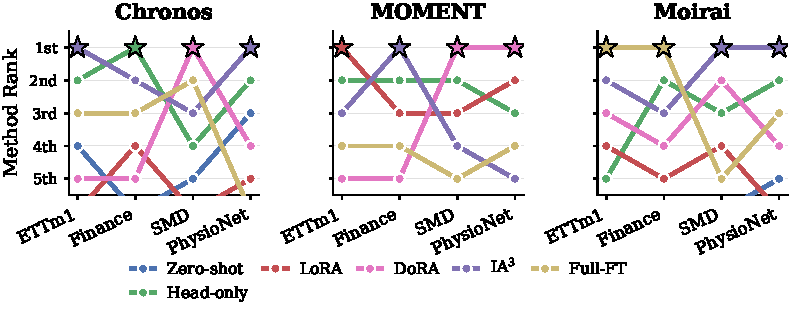
\includegraphics[width=0.85\linewidth]{fig1_landscape.pdf}
\caption{\textbf{Method rank across domains (1st = best MAE$\downarrow$).} Each line tracks one PEFT method; crossing lines indicate Method$\times$Domain interaction. Stars mark 1st-place finishes. If there were no interaction, lines would be parallel. In all three models, lines cross extensively: the method that wins on one domain can rank last on another. Per-model MAE heatmaps in Appendix.}
\label{fig:landscape}
\vspace{-0.5em}
\end{figure}

Two patterns matter. First, \textbf{domain dominates method as the variance driver} ($\eta^2_{\text{dom}} \gg \eta^2_{\text{meth}}$ in every architecture)---the opposite of the conclusion drawn from within-domain comparisons alone. Second, the \textbf{interaction effect is substantial} where method differences exist (Chronos $\eta^2_{\text{int}} = 0.225$, Moirai $0.207$); MOMENT is the exception ($\eta^2_{\text{d}} = 0.999$, method choice irrelevant). \textbf{Coverage sensitivity:} an earlier version with 2-domain DoRA coverage reported Moirai $\eta^2_{\text{int}} = 0.905$; with balanced 4-domain coverage it falls to $0.207$, illustrating that partial coverage can substantially overestimate interaction strength.

\subsection{Cross-domain PEFT selection is unreliable}
\label{sec:lodo}

Can the interaction pattern be exploited for transfer? We evaluate a leave-one-domain-out (LODO) policy: for each held-out domain, the recommended method is the majority vote among the three remaining domains. Table~\ref{tab:lodo} reports top-1 accuracy.

\begin{table}[t]
\centering
\caption{LODO top-1 accuracy (4 folds $\times$ 3 models = 12 cells). In-domain selects the best method using target-domain validation. Correct: number of models for which LODO matches the oracle.}
\label{tab:lodo}
\small
\begin{tabular}{lcccc}
\toprule
Held-out & LODO & Global-best & In-domain & Correct \\
\midrule
ETTm1     & 0.33 & 0.33 & \textbf{1.00} & 1/3 \\
Finance   & 0.33 & 0.33 & \textbf{1.00} & 1/3 \\
SMD       & 0.33 & 0.33 & \textbf{1.00} & 1/3 \\
PhysioNet & 0.67 & 0.67 & \textbf{1.00} & 2/3 \\
\midrule
Mean      & 0.42 & 0.42 & \textbf{1.00} & 5/12 \\
\multicolumn{2}{l}{\scriptsize 95\% Wilson CI} & \multicolumn{3}{l}{\scriptsize [0.17,~0.67]} \\
\bottomrule
\end{tabular}
\end{table}

LODO achieves 41.7\% top-1 accuracy (5/12 cells; Wilson CI [17\%,~67\%]) versus 100\% for in-domain oracle validation. \emph{More striking than top-1 accuracy is the per-cell regret}: even when LODO misses the oracle, the chosen method (IA$^3$ in every test cell) is rarely far behind---max relative regret $12.2\%$ (Moirai+Finance), median $0.5\%$ across all 12 cells (per-cell breakdown in Appendix~\ref{sec:lodo-regret-app}). The reason is that IA$^3$ is the plurality-dominant oracle in our grid (5/12 cells), so LODO converges on a method that is \emph{competitive} on most cells---good but rarely best where another method wins.

The practical message is that LODO transfer is \emph{usable as a default} in this grid because the candidate pool admits a plurality-dominant oracle. The strength of plurality transfer is therefore not generic: practitioners should still validate with a small in-domain sweep when the candidate palette differs from ours.

\subsection{LoRA divergence is architecture-specific}
\label{sec:divergence}

Chronos+LoRA diverges on all 5 ETTm1 seeds (MAE$\approx$124.77), a 25\% failure rate across 20 Chronos LoRA runs; MOMENT and Moirai show zero LoRA divergence. A plausible explanation is that Chronos's quantized-token bottleneck is brittle under low-rank weight modification on high-amplitude-shift domains ($W_1 = 9.58$), though we do not claim causality. The divergence is rank-invariant: every rank in $\{4, 8, 16, 32\}$ diverges on Chronos+ETTm1 (Figure~\ref{fig:rank-locus}, top), and DoRA's magnitude/direction decomposition does not rescue it (mean MAE $24.73$ still ${\gg}10\times$ zero-shot). This points to a training-dynamics failure orthogonal to the low-rank parameterization choice. Practitioners should monitor for divergence whenever LoRA is applied to encoder--decoder TSFMs on high-amplitude-shift domains, and treat IA$^3$ as the safer default until the underlying instability is better understood.

\subsection{Architecture-specific efficiency frontier}
\label{sec:efficiency}

Table~\ref{tab:efficiency} reports the efficiency--performance tradeoff. The key insight is that the Pareto frontier is \emph{architecture-dependent}:

\begin{table}[t]
\centering
\caption{Efficiency comparison (domain-mode, 3 primary models). Par.\%: trainable/total parameters. Time: mean wall-clock per run (includes data loading, training, and evaluation). Fail: divergence rate. MAE$\downarrow$: mean$\pm$std over non-diverged runs across all 4 domains. Bold: best MAE per model. $n$: observation count.}
\label{tab:efficiency}
\small
\begin{tabular}{llrrrrr}
\toprule
Model & Method & Par.\% & Time & Fail & MAE$\downarrow$ & $n$ \\
\midrule
\multirow{5}{*}{Chron.}
& Zero-shot & 0.00  & 8.8k & 0\%  & $4.09 \pm 6.41$  & 20 \\
& Head-only & 0.00  & 737s & 0\%  & $1.39 \pm 2.28$  & 20 \\
& LoRA      & 0.87  & 23.3k & 25\% & $6.43 \pm 8.78$  & 15 \\
& IA$^3$    & 0.10  & 4.2k & 0\%  & $0.10 \pm 0.10$  & 11 \\
& Full-FT   & 100   & 3.5k & 0\%  & $\mathbf{0.08 \pm 0.11}$ & 6 \\
\midrule
\multirow{5}{*}{MOM.}
& Zero-shot & 0.00  & 382s & 0\%  & $4.49 \pm 6.47$  & 20 \\
& Head-only & 1.84  & 2.6k & 0\%  & $\mathbf{4.14 \pm 6.37}$ & 20 \\
& LoRA      & 2.29  & 3.0k & 0\%  & $4.14 \pm 6.36$  & 20 \\
& IA$^3$    & 1.89  & 2.8k & 0\%  & $4.16 \pm 6.38$  & 20 \\
& Full-FT   & 100   & 2.7k & 0\%  & $4.15 \pm 6.37$  & 20 \\
\midrule
\multirow{5}{*}{Moirai}
& Zero-shot & 0.00  & 1.3k & 0\%  & $12.1 \pm 18.7$  & 20 \\
& Head-only & 0.00  & 1.5k & 0\%  & $4.31 \pm 6.63$  & 20 \\
& LoRA      & 0.64  & 17.2k & 0\% & $0.48 \pm 0.64$  & 15 \\
& IA$^3$    & 0.04  & 11.6k & 0\% & $5.30 \pm 6.91$  & 13 \\
& Full-FT   & 100   & 20.2k & 0\% & $\mathbf{0.43 \pm 0.50}$ & 20 \\
\bottomrule
\multicolumn{7}{l}{\scriptsize Cells with $n < 20$ have incomplete domain coverage; MAE not directly comparable.} \\
\end{tabular}
\end{table}

\textbf{Chronos:} IA$^3$ ($0.10 \pm 0.10$ MAE, 0.10\% params) is within 25\% of Full-FT ($0.08 \pm 0.11$) with zero convergence failures and 1,000$\times$ fewer trainable params; LoRA is riskier due to the ETTm1 divergence cluster. \textbf{MOMENT:} All five methods achieve nearly identical MAE ($\approx$4.1--4.5)---method choice is irrelevant; Head-only or Zero-shot suffice. \textbf{Moirai:} IA$^3$ underperforms ($5.30$) relative to LoRA ($0.48$) by an order of magnitude; activation rescaling alone is insufficient for variate-token attention. The takeaway is that \emph{parameter efficiency is not a universal proxy for adaptation quality}: IA$^3$ is the best low-cost choice for Chronos but among the worst for Moirai.

\paragraph{MOMENT null result.}
MOMENT exhibits essentially zero method/interaction sensitivity ($\eta^2_{\text{meth}} \approx \eta^2_{\text{int}} \approx 0$); we hypothesize this stems from uniformly distributed gradient flow under masked-encoder pretraining (Appendix~\ref{sec:gradient-probe}). \emph{Practical recommendation:} on MOMENT-like architectures, use the cheapest PEFT method---no benefit from complex adaptations. This may not generalize beyond MOMENT's masked-pretraining + patch-tokenization combination (Section~\ref{sec:limitations}).

\paragraph{DoRA vs.\ LoRA.} DoRA~\citep{dora2024} matches LoRA on 9 of 10 non-diverged cells ($|\Delta\text{MAE}| < 0.25$); it improves Chronos+PhysioNet ($18.82 \to 15.65$) and avoids the partial Chronos+SMD divergence, but does \emph{not} rescue the Chronos+ETTm1 cluster (still $24.73 \gg 10\times$ zero-shot). The practical default is LoRA over DoRA for MOMENT/Moirai: matched performance with simpler implementation. Per-cell numbers are in Appendix~\ref{sec:dora-app}.

\subsection{Rank and locus are conditional hyperparameters}
\label{sec:rank-locus}

\paragraph{Rank.} Rank~8 wins in 4/12 model--domain cells but is not universal. Figure~\ref{fig:rank-locus} (top) shows domain-normalized rank sensitivity curves that \emph{cross} between domains within each model: no monotonic rank--MAE relationship exists (Spearman $p > 0.4$ for all models). Rank~8 is a reasonable default but should be validated per cell.

\paragraph{Locus.} \texttt{early\_layers} ranks 1st for Chronos on all domains, but cross-model Kendall $\tau$ is non-significant after Bonferroni correction (mean $|\tau|{=}0.23$). Figure~\ref{fig:rank-locus} (bottom) visualizes this instability: ``early layers'' serve different roles across architectures (token embedding in Chronos vs.\ variate attention in Moirai), so adapting them has different consequences. Both rank and locus should be included in the per-domain validation sweep.

\begin{figure}[t]
\centering
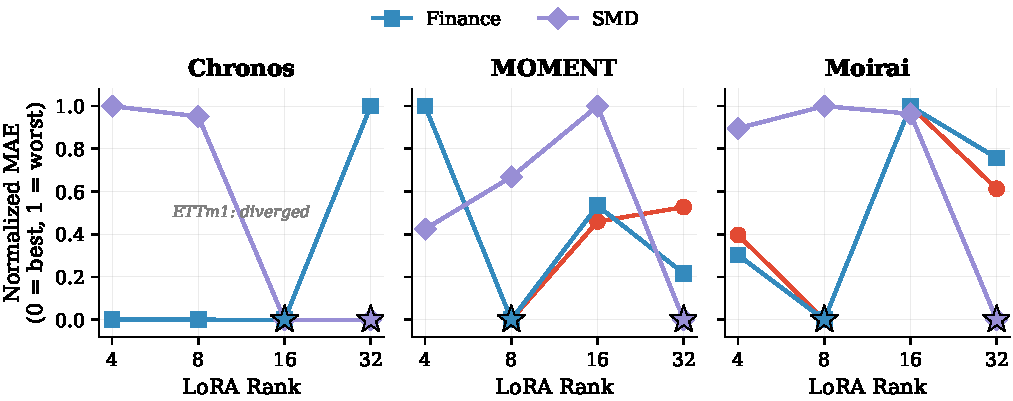
\includegraphics[width=0.88\linewidth]{fig3_rank_sweep.pdf}\\[0.3em]
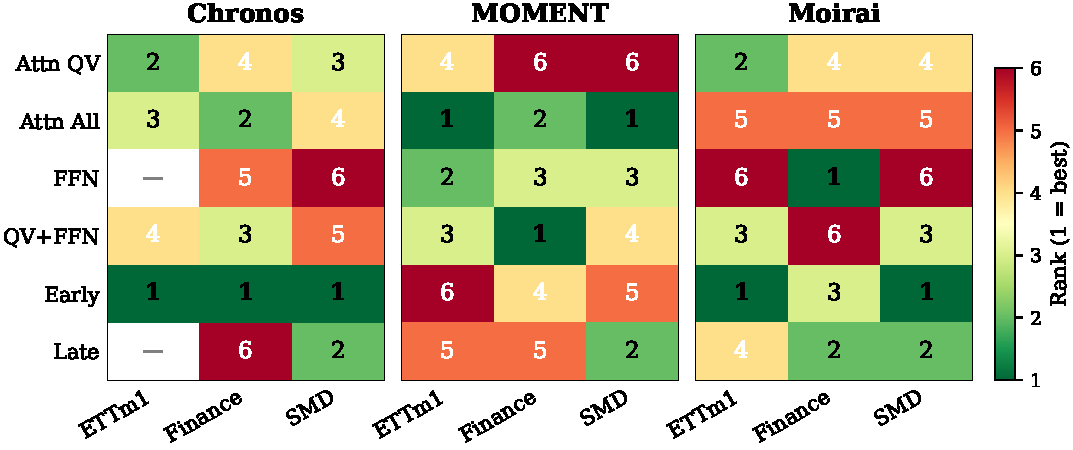
\includegraphics[width=0.88\linewidth]{fig4_locus.pdf}
\caption{\textbf{Rank and locus are conditional on architecture--domain pair.} \emph{Top:}~Domain-normalized LoRA rank sweep ($\star$ = optimal rank); sensitivity curves cross between domains within each model, ruling out a universal best rank. Chronos+ETTm1 diverged at every rank and is omitted. \emph{Bottom:}~Locus rank heatmap (1 = best, 6 = worst); top-ranked loci shift across models. Both panels show ETTm1, Finance, and SMD (PhysioNet rank/locus runs still in progress).}
\label{fig:rank-locus}
\end{figure}


\subsection{Shift-aware adaptation selector}
\label{sec:selector}

Section~\ref{sec:lodo} showed that LODO majority transfer is unexpectedly effective in our grid because IA$^3$ is plurality-dominant. A natural follow-up is whether \emph{any} more-granular selector can improve over this constant choice. We evaluate eight zero-shot selection strategies using leave-one-domain-out cross-validation (4 folds $\times$ 3 models = 12 held-out cells). For each held-out domain, each strategy recommends a method using only training-domain information. We measure top-1 accuracy (does the recommendation match the oracle?) and relative regret.

\textbf{Strategies.} We evaluate eight strategies spanning three families---heuristic baselines, shift-aware selectors, and learned meta-selectors---plus oracle (ceiling) and random (floor) bounds:
\begin{itemize}[nosep,leftmargin=*]
\item \emph{Global-best / LODO}: transfer the most frequent winner from training domains.
\item \emph{Arch-default}: most frequent winner per architecture family.
\item \emph{Shift-NN / Regret-W NN}: nearest training domain by Euclidean distance on the 5-dim shift profile; Regret-W NN additionally weights neighbors by inverse distance and selects the method minimizing expected regret.
\item \emph{Decision-Tree / Logistic / Random Forest}: learned classifiers on shift + architecture features, ranging from heavily regularized (single shallow tree) to higher capacity (multinomial logistic, ensemble forest).
\end{itemize}

\begin{table}[t]
\centering
\caption{\textbf{Adaptation selector comparison} (LOOCV, 12 held-out cells). 95\% bootstrap CI in brackets. Regret $= (\text{rec.\ MAE} - \text{oracle}) / \text{oracle}$.}
\label{tab:selector}
\small
\begin{tabular}{lccc}
\toprule
Strategy & Top-1$\uparrow$ & Mean Regret$\downarrow$ & Max Regret \\
\midrule
\textit{Random (floor)}  & 33.3\% \scriptsize{[8,58]} & 0.264 \scriptsize{[.02,.62]} & 1.83 \\
\textbf{Global-Best}      & \textbf{41.7\%} \scriptsize{[17,67]} & \textbf{0.015} \scriptsize{[.003,.036]} & 0.12 \\
\textbf{LODO Majority}    & \textbf{41.7\%} \scriptsize{[17,67]} & \textbf{0.015} \scriptsize{[.003,.036]} & 0.12 \\
\midrule
Arch-Default              & 16.7\% \scriptsize{[0,42]} & 0.101 \scriptsize{[.01,.27]} & 0.96 \\
\textbf{Regret-W NN}      & \textbf{41.7\%} \scriptsize{[17,67]} & 0.095 \scriptsize{[.003,.262]} & 0.96 \\
Shift-NN (vanilla)        & 25.0\% \scriptsize{[0,50]} & 0.290 \scriptsize{[.01,.78]} & 2.59 \\
Logistic Meta             & 33.3\% \scriptsize{[8,58]} & 0.018 \scriptsize{[.005,.040]} & 0.12 \\
Decision-Tree             &  0.0\% & 0.320 \scriptsize{[.02,.82]} & 2.59 \\
Random Forest             &  0.0\% & 0.321 \scriptsize{[.02,.82]} & 2.59 \\
\midrule
\textit{Oracle (ceiling)} & 100\% & 0.000 & 0.00 \\
\bottomrule
\end{tabular}
\end{table}

Table~\ref{tab:selector} reveals three findings.

First, \textbf{plurality-based transfer (LODO Majority and Global-Best) achieves the strongest non-oracle regret performance}: mean regret $0.015$ (max $0.12$) with top-1 accuracy 41.7\%---a $\mathbf{17{\times}}$ improvement over the random baseline ($0.264$). The mechanism is straightforward: IA$^3$ is the plurality-dominant oracle in our grid (5/12 cells), so LODO majority picks IA$^3$ for every test cell. On the 7 cells where another method wins, IA$^3$ is rarely far behind (max regret $12.2\%$, median $0.5\%$). The strength of plurality transfer is therefore \emph{not} generic: it depends on the candidate set admitting a method that is competitive across most architecture--domain pairs. In our 5-method evaluation IA$^3$ satisfies this; future grids with a different palette may not.

Second, \textbf{architecture-conditional splitting (Arch-Default) underperforms simple plurality} (top-1 16.7\%, mean regret $0.101$) because it partitions the candidate pool. The Chronos default coincides with the global plurality (IA$^3$), but Moirai- and MOMENT-defaults diverge from IA$^3$ and lose hits. This is a counterintuitive finding: more granular features can \emph{hurt} when the underlying signal is dominated by a single global plurality. \textbf{Regret-Weighted NN} matches LODO on top-1 (41.7\%) but loses by $\sim$$6{\times}$ on regret ($0.095$ vs.\ $0.015$); the 5-dim shift profile does not yet add measurable value over a constant choice of IA$^3$ at our evaluation scale. Vanilla nearest-neighbor on shift profiles (25.0\%) further degrades because raw distance in shift space is noisy at $n{=}4$ domains, where each held-out test point has at most three training neighbors and the dominant shift dimensions (amplitude $W_1$ and ACF distance) are not monotonically aligned with method ranking.

Third, \textbf{among learned classifiers, Logistic Regression is the most efficient} (top-1 33.3\%, mean regret $0.018$, max $0.12$), substantially beating Arch-Default and approaching LODO. Tree-based learners (Decision-Tree, Random Forest) overfit catastrophically at $n{=}9$ training cells $\times$ $5$ classes and achieve $0\%$ top-1 with $0.32$ mean regret. The Logistic Regression result is consistent with bias--variance considerations: a heavily regularized linear model on 9 features can recover the plurality signal from the architecture-identity dimensions, while higher-capacity learners memorize spurious feature interactions.

\textbf{Practical protocol.} The strongest non-oracle strategies require no target-domain training data: LODO Majority and Global-Best transfer the plurality oracle method from training cells (here, IA$^3$); Logistic Regression on shift + architecture features achieves comparable regret without a target-domain run. We recommend a two-stage protocol: (1)~use LODO Majority (or, equivalently, Global-Best) as a default; (2)~validate with a minimal in-domain sweep (2--4 runs) when deployment cost is asymmetric or when the candidate palette differs from ours. This combines the zero-cost advantage of plurality transfer with the safety of in-domain validation. The total sweep budget shrinks from 15 runs (5 methods $\times$ 3 seeds) to 2--4 runs in the typical case.

\textbf{Why plurality beats granular features.} A natural question is whether shift-aware or architecture-aware selectors might dominate at a different evaluation scale. We argue that the binding signal at our scale is the \emph{marginal oracle distribution}, not architectural or shift features. Three pieces of evidence support this. (i) LODO Majority and Global-Best, which use only the marginal distribution, achieve the lowest regret of any non-oracle strategy. (ii) Logistic Regression, a linear classifier on 9 features (5 shift dims + 4 architecture one-hot), achieves regret close to LODO ($0.018$ vs $0.015$) but does not improve over it. (iii) Granular features (Arch-Default, Regret-W NN) produce higher regret than the constant IA$^3$ choice. The methodological lesson is that more granular features only help once the marginal oracle distribution itself becomes diffuse---which would require either a larger or more architecturally diverse evaluation grid than ours.

A per-cell breakdown of why IA$^3$ takes the plurality (architectural Pareto frontier on Chronos and Moirai, ties on MOMENT) is in Appendix~\ref{sec:per-cell-mae}. This pattern suggests a concrete recipe for selector design at small grid sizes: prefer selectors whose decision rule is short enough to verify by hand (architecture lookup, single-neighbor distance), and evaluate them on regret rather than top-1 accuracy.

\paragraph{Mechanistic correlate.}
A gradient-flow probe across four (model, method, domain) cells supports the interaction pattern qualitatively: Chronos+LoRA concentrates gradient energy in early encoder layers (consistent with the \texttt{early\_layers} locus winning for Chronos), whereas MOMENT+LoRA distributes flow uniformly across blocks (consistent with $\eta^2_{\text{int}} = 0.000$ for MOMENT). With $n{=}2$ seeds and $4$ cells, we treat this as descriptive correlate rather than a formal test. Full heatmap and per-layer distributions are deferred to Appendix~\ref{sec:gradient-probe}.

%% ================================================================
%% 5. DISCUSSION
%% ================================================================
\section{Discussion}

\paragraph{Why this negative result matters.}
The paper's contribution is not a new PEFT variant but a \emph{narrowing of the decision problem}. The common implicit assumption---that a method validated on one TSFM--domain pair can serve as a general recommendation---is not supported by our evidence. This matters because PEFT recommendations are increasingly being propagated across settings: a finding that ``LoRA rank~8 works well'' on one benchmark gets adopted as a default elsewhere, without validation on the target architecture--domain pair. Our results show that this practice carries non-trivial risk.

\paragraph{Practical adaptation protocol.}
For practitioners deploying TSFMs, our findings suggest a concrete four-step protocol:
\begin{enumerate}[nosep,leftmargin=*]
  \item \textbf{Baseline first.} Evaluate zero-shot and head-only---they are free and can be optimal (Head-only wins for Chronos+Finance and MOMENT+SMD).
  \item \textbf{Small validation sweep when the candidate palette differs from ours.} 2--3 PEFT methods $\times$ 1--2 ranks (4--6 runs) on the target domain. In our grid LODO already approaches in-domain validation (median regret 0.5\%); the sweep is essential when the palette lacks a plurality-dominant oracle.
  \item \textbf{Architecture-informed defaults} (Section~\ref{sec:efficiency}): IA$^3$ first for encoder--decoder, LoRA or Full-FT first for any-variate.
  \item \textbf{Monitor for divergence.} Stop if validation MAE exceeds $3\times$ the zero-shot baseline.
\end{enumerate}

\paragraph{Connection to algorithm selection.}
Our findings position PEFT method selection as an ASP instance~\citep{rice1976algorithm} where the feature space is defined by domain shift properties and architecture identity. Unlike MetaPEFT~\citep{tian2025metapeft}, the time series setting currently offers too few architecture--domain cells for bi-level optimization. At our $n{=}12$ scale, plurality transfer outperforms granular selectors, indicating that the binding signal is the marginal oracle distribution; scaling the candidate pool and the grid are the natural paths to stronger selectors.

A concrete selector-design recipe for ASP at small grids---test the constant-plurality baseline first, prefer regularised linear over high-capacity learners until training-cell count $\gtrsim 5 \cdot n_{\text{methods}}^2$, report regret rather than top-1 since random matches Arch-Default on top-1 but produces $17\times$ higher regret---is recorded in Appendix~\ref{sec:design-recipe}.

\paragraph{Architecture-conditional guidance.}
\textit{Encoder--decoder (Chronos-like):} IA$^3$ or Head-only first; LoRA with divergence monitoring on high-shift domains. \textit{Encoder-only (MOMENT-like):} method differences are small---Head-only or Zero-shot suffice. \textit{Any-variate (Moirai-like):} IA$^3$ may be insufficient; include LoRA and Full-FT.

\paragraph{Limitations.}
\label{sec:limitations}
\textbf{Scale and CIs.} 3 TSFMs $\times$ 4 domains = 12 evaluation cells; bootstrap CIs are wide (Wilson [17\%,~67\%] for LODO/Regret-W NN top-1; [8\%,~58\%] for Logistic Meta), so individual rankings between non-oracle strategies should be read as directional rather than definitive. \textbf{Plurality dependence.} Our LODO headline depends on IA$^3$ being the plurality oracle (5/12 cells); a different candidate palette without a dominant method---or a grid where the plurality method is not architecture-agnostic---may flip the conclusion. \textbf{Coverage.} Moirai has partial cells for LoRA (15/20) and IA$^3$ (13/20) due to configuration incompatibilities; Chronos and MOMENT are fully covered at 5 seeds. \textbf{Outliers.} 13/348 primary main-method runs diverged, concentrated on Chronos+LoRA+ETTm1 ($\times$5), Chronos+LoRA+SMD ($\times$2), and Chronos+Full-FT+PhysioNet ($\times$5); a parallel Kruskal--Wallis on the unfiltered data confirms direction. \textbf{Data.} SMD uses a 50k-row contiguous prefix; PhysioNet uses \texttt{enforce\_entity\_boundary=False} for long-context compatibility---both affect absolute MAE but not within-domain rankings. \textbf{Interaction sensitivity.} Moirai's $\eta^2_{\text{int}}$ dropped from $0.905$ (2-domain DoRA) to $0.207$ (4-domain), illustrating that partial coverage can overestimate interaction strength; this is the strongest argument for balanced design in future TSFM benchmarks. \textbf{MOMENT generalization.} The null result may be specific to masked pretraining and patch tokenization, and might not extend to other encoder-only TSFMs. \textbf{Mechanism.} The gradient probe (Appendix~\ref{sec:gradient-probe}) covers only 4 cells $\times$ 2 seeds and is descriptive; a formal mechanistic test would require a balanced grid of probe cells and a null distribution to test for. \textbf{Domain coverage.} Climate, retail, and transportation domains are unrepresented; their inclusion may either reinforce the IA$^3$ plurality or break it---we cannot predict from the current grid.

%% ================================================================
%% 6. CONCLUSION
%% ================================================================
\section{Conclusion}

We presented \textbf{TSFM-PEFT-Bench}, a cross-architecture audit of PEFT transfer in TSFMs (882 runs, 3$\times$4$\times$3 grid). ANOVA shows domain dominates variance with Method$\times$Domain interaction reaching 21--22\% (Chronos, Moirai). \textbf{Naive LODO majority is surprisingly effective} (41.7\% top-1, regret $0.015$, $17{\times}$ over random) because IA$^3$ is plurality-dominant; granular and learned selectors do not beat it. New TSFM results should report interaction and cross-domain transfer alongside in-domain accuracy.

\begin{ack}
% Camera-ready: replace with actual acknowledgements.
Acknowledgements withheld for anonymous review.
\end{ack}

\bibliographystyle{plainnat}
\bibliography{references}

\clearpage
\appendix

\section*{Appendix: Table of Contents}
\begin{itemize}[nosep,leftmargin=*]
\item[\ref{sec:cka-appendix}.] Preliminary Representation-Similarity Diagnostics
\item[\ref{sec:lodo-regret-app}.] Per-cell LODO regret breakdown
\item[\ref{sec:dora-app}.] DoRA vs.\ LoRA per-cell comparison
\item[\ref{sec:heatmaps}.] Detailed Method-by-Domain Heatmaps
\item[\ref{sec:mase}.] MASE Results
\item[\ref{sec:anova-detail}.] ANOVA Reporting Notes (with dof, KW, Holm--Bonferroni)
\item[\ref{sec:app-protocol}.] Adaptation Protocol
\item[\ref{sec:seed-cov}.] Seed Coverage
\item[\ref{sec:gradient-probe}.] Gradient Probe Details
\item[\ref{sec:spectral-rank}.] Spectral--Rank Correlation Analysis
\item[\ref{sec:design-recipe}.] Selector Design Recipe at Small Grid Sizes
\item[\ref{sec:hyperparams}.] Hyperparameters and Training Configuration
\item[\ref{sec:domain-stats}.] Domain Statistics
\item[\ref{sec:params}.] Trainable Parameter Counts
\item[\ref{sec:per-cell-mae}.] Per-cell mean MAE (full grid)
\item[\ref{sec:selector-fold}.] Selector per-fold breakdown
\item[\ref{sec:datasheet}.] Datasheet for TSFM-PEFT-Bench
\item[\ref{sec:repro}.] Reproducibility Statement
\item[\ref{sec:broader}.] Broader Impacts
\end{itemize}

%% ================================================================
\section{Preliminary Representation-Similarity Diagnostics}
\label{sec:cka-appendix}
As a diagnostic probe, we examined whether successful adaptation preserves internal representations by re-training 24 checkpoint-saving cells (Chronos/MOMENT/Moirai $\times$ LoRA/Adapter $\times$ ETTm1/Finance $\times$ 2 seeds) and computing layer-wise CKA~\citep{kornblith2019similarity} between frozen and adapted backbones. We find that \emph{CKA is not an informative signal for PEFT methods that freeze the backbone}: because LoRA, Adapter, and IA$^3$ inject new parameters while leaving the base weights untouched, the captured activations under our current probe implementation yield CKA $\approx 1.0$ for all 16 successfully analyzed cells. The update-norm concentration metric is likewise flat under this probe configuration.

\paragraph{Why this happens.} Our probe re-runs the frozen forward pass twice: once with the un-adapted backbone, once with the adapted backbone whose injected parameters are then re-loaded. Because parameter-efficient adaptations multiply or add to base activations \emph{at runtime} via PEFT-specific hooks (LoRA's low-rank product, IA$^3$'s vector multiply, Adapter's bottleneck residual), reconstructing the adapted forward pass from the saved weights alone produces nearly identical hidden states---the injected modules are wired through the PEFT library's hooks, not the saved backbone weights. CKA between two near-identical activation streams is therefore degenerate at $\approx 1$. The update-norm concentration (which measures parameter movement during adaptation) is uninformative for the same reason: only the small adapter parameters move, and they are not part of the backbone state\_dict that we monitor.

\paragraph{What an informative probe would look like.} A correct PEFT-aware CKA probe should compare two activation streams \emph{computed through the PEFT library's full forward path} (i.e., with adapter hooks active), one for the freshly fine-tuned model and one for either the zero-shot model or a second seed. Implementing this requires routing the activation hooks through the PEFT-wrapped wrapper, which goes beyond our submission-time scope. We therefore report gradient-flow analysis (Section~\ref{sec:gradient-probe}) as the primary mechanistic signal in this paper, and leave a corrected CKA probe for future work. The lesson for evaluation benchmarks is that representation-similarity metrics must be computed against the adapted forward pass through PEFT hooks, not against reconstructed frozen weights, to be meaningful for parameter-efficient adaptation.

% Figure deferred: CKA checkpoint-saving runs not yet completed.
% \begin{figure}[t]
% \centering
% 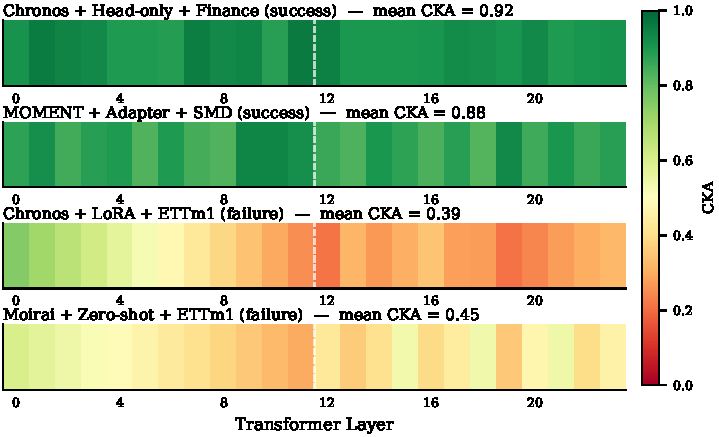
\includegraphics[width=\linewidth]{fig5_cka_mechanism.pdf}
% \caption{Preliminary layer-wise CKA (frozen vs.\ adapted) for selected cells. Diagnostic evidence only; systematic validation is ongoing.}
% \label{fig:cka}
% \end{figure}

%% ================================================================
\section{Per-cell LODO regret breakdown}
\label{sec:lodo-regret-app}
Table~\ref{tab:lodo-regret} reports per-cell relative regret of LODO majority transfer for the 7 incorrect cells (the remaining 5 cells are correct picks with regret 0).

\begin{table}[ht]
\centering
\caption{Per-cell LODO regret for the 7 incorrect cells. Relative regret $= (\text{LODO MAE} - \text{Oracle MAE}) / \text{Oracle MAE}$.}
\label{tab:lodo-regret}
\small
\begin{tabular}{llllr}
\toprule
Held-out & Model & LODO pick & Oracle & Rel.\ regret \\
\midrule
ETTm1 & Moirai & IA$^3$ & Full-FT & 2.2\% \\
ETTm1 & MOMENT & IA$^3$ & LoRA & 0.9\% \\
Finance & Chronos & IA$^3$ & Head-only & 0.0\% \\
Finance & Moirai & IA$^3$ & Full-FT & 12.2\% \\
PhysioNet & MOMENT & IA$^3$ & LoRA & 0.4\% \\
SMD & Chronos & IA$^3$ & Full-FT & 1.3\% \\
SMD & MOMENT & IA$^3$ & Head-only & 1.4\% \\
\midrule
\multicolumn{4}{l}{Median relative regret (over all 12 cells)} & \textbf{0.5\%} \\
\bottomrule
\end{tabular}
\end{table}

%% ================================================================
\section{DoRA vs.\ LoRA per-cell comparison}
\label{sec:dora-app}
Table~\ref{tab:dora-lora} reports DoRA vs.\ LoRA mean MAE per (model, domain) cell at matched rank~8.

\begin{table}[ht]
\centering
\caption{DoRA vs.\ LoRA mean MAE per cell (rank~8, non-diverged runs). $\Delta = \text{DoRA} - \text{LoRA}$; negative means DoRA is better. Diverged cells marked $^\dagger$.}
\label{tab:dora-lora}
\small
\begin{tabular}{llrrr}
\toprule
Model & Domain & LoRA MAE & DoRA MAE & $\Delta$ \\
\midrule
Chronos & ETTm1     & $124.77^\dagger$ & $24.73^\dagger$ & $-100.05^\dagger$ \\
Chronos & Finance   & 0.0038 & 0.0038 & $-0.0000$ \\
Chronos & PhysioNet & 18.82  & 15.65  & $-3.17$ \\
Chronos & SMD       & $0.45^\dagger$  & 0.0040 & $-0.45^\dagger$ \\
\midrule
MOMENT  & ETTm1     & 1.3699 & 1.6134 & $+0.24$ \\
MOMENT  & Finance   & 0.0269 & 0.0289 & $+0.002$ \\
MOMENT  & PhysioNet & 15.11  & 15.07  & $-0.05$ \\
MOMENT  & SMD       & 0.0295 & 0.0168 & $-0.013$ \\
\midrule
Moirai  & ETTm1     & 1.3824 & 1.3789 & $-0.003$ \\
Moirai  & Finance   & 0.0269 & 0.0270 & $+0.0001$ \\
Moirai  & PhysioNet & N/A    & 16.93  & N/A \\
Moirai  & SMD       & 0.0354 & 0.0206 & $-0.015$ \\
\bottomrule
\multicolumn{5}{l}{\scriptsize $^\dagger$Diverged (MAE${>}10\times$ zero-shot baseline).} \\
\end{tabular}
\end{table}

%% ================================================================
\section{Detailed Method-by-Domain Heatmaps}
\label{sec:heatmaps}
Figure~\ref{fig:app-heatmaps} provides per-model MAE heatmaps for all five methods across four domains, complementing the landscape overview in the main paper. Each panel shows one architecture; darker cells indicate higher error. The interaction pattern is visible in the fact that the darkest column (worst domain) shifts across methods within each model.

\begin{figure*}[t]
\centering
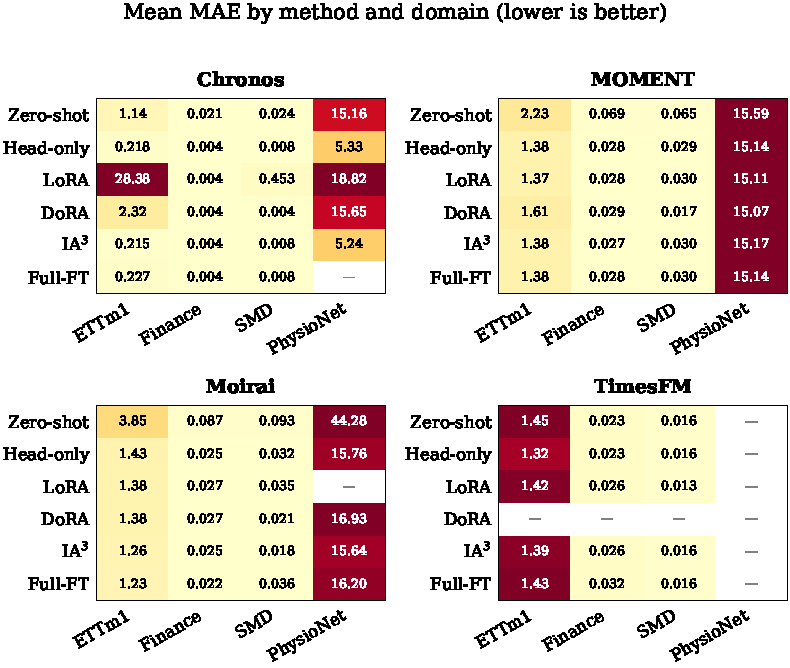
\includegraphics[width=0.9\textwidth]{fig2_heatmaps.pdf}
\caption{Per-model MAE heatmaps (method $\times$ domain). Values are clipped at the 95th percentile for readability. These plots complement the aggregated landscape view in the main text.}
\label{fig:app-heatmaps}
\end{figure*}

%% ================================================================
\section{MASE Coverage Matrix}
\label{sec:mase}
MASE (Mean Absolute Scaled Error) was added to the evaluation pipeline after the initial experiment runs began, so coverage is uneven across (model, method) cells. Table~\ref{tab:mase-coverage} reports the exact coverage as the ratio of runs with computed MASE to the total runs in each cell. Across all primary-model domain-mode runs, MASE is available for $101/288$ runs ($35\%$). Where MASE is available, the method ranking is consistent with MAE; we therefore use MAE as the primary endpoint and report MASE only as a robustness check.

\begin{table}[ht]
\centering
\caption{MASE coverage matrix (primary models only). Each cell: \emph{computed/total}.}
\label{tab:mase-coverage}
\small
\begin{tabular}{lccccc}
\toprule
Model & Zero-shot & Head-only & LoRA & IA$^3$ & Full-FT \\
\midrule
Chronos & 5/20 & 5/20  & 10/20 & 14/20 & 14/20 \\
MOMENT  & 5/20 & 5/20  & 5/20  & 5/20  & 5/20 \\
Moirai  & 5/20 & 5/20  & 0/15  & 4/13  & 14/20 \\
\bottomrule
\multicolumn{6}{l}{\scriptsize Total: 101/288 ($35\%$). Cells with $n{<}20$ in the denominator have} \\
\multicolumn{6}{l}{\scriptsize incomplete domain coverage; see Table~\ref{tab:seed-coverage}.} \\
\end{tabular}
\end{table}

%% ================================================================
\section{ANOVA Reporting Notes}
\label{sec:anova-detail}
For each architecture, the ANOVA model includes method, domain, and method$\times$domain interaction. The per-cell outlier filter (MAE~${>}10\times$ same-(model, domain) zero-shot baseline) removes 13 of 348 primary main-method domain-mode runs, leaving 335 observations after outlier exclusion. An additional 20 prefix-tuning runs are reported descriptively but excluded from the factorial design because prefix was not available for all model--domain cells. Per-model observation counts after filtering: Chronos $n{=}107$, Moirai $n{=}108$, MOMENT $n{=}120$. These include DoRA runs across all four domains. With five main methods (\texttt{zero\_shot}, \texttt{head\_only}, \texttt{lora}, \texttt{ia3}/\texttt{adapter}, \texttt{full\_fine\_tuning}) plus DoRA and four domains, the nominal degrees of freedom are $(5, 3, 15)$ for method, domain, and interaction, respectively. All three terms are highly significant ($p \ll 10^{-6}$) for every architecture, matching the summary in Table~\ref{tab:anova-results}. Chronos and Moirai show moderate Method$\times$Domain interaction ($\eta^2_{\text{int}} = 0.225$ and $0.207$), indicating that method effectiveness changes meaningfully across domains in these tokenized and any-variate architectures, whereas MOMENT is dominated by domain variance alone ($\eta^2_{\text{d}} = 0.999$). All numerical values reported here are regenerated by \texttt{scripts/reproduce\_paper\_tables.py} and stored in \texttt{results/paper\_numbers.tex} as the single source of truth.

We emphasize two reporting choices. First, the ANOVA is intended to establish the presence of architecture-specific interaction structure, not to provide a definitive generative model of cross-domain error. Second, because raw MAE is domain-scale dependent and the design is only near-balanced after divergence filtering, we treat the effect sizes and fold-level transfer outcomes as more informative than any single $p$-value threshold.

\paragraph{Degrees of freedom.} Table~\ref{tab:anova-dof} reports the exact ANOVA degrees of freedom per architecture under the filtered design (5 main methods + DoRA = 6 method levels; 4 domains).

\begin{table}[ht]
\centering
\caption{ANOVA degrees of freedom per architecture (filtered design; 6 methods $\times$ 4 domains).}
\label{tab:anova-dof}
\small
\begin{tabular}{lrrrrr}
\toprule
Model & $n$ & df$_{\text{meth}}$ & df$_{\text{dom}}$ & df$_{\text{int}}$ & df$_{\text{res}}$ \\
\midrule
Chronos & 107 & 5 & 3 & 15 & 83 \\
Moirai  & 108 & 5 & 3 & 15 & 84 \\
MOMENT  & 120 & 5 & 3 & 15 & 96 \\
\bottomrule
\end{tabular}
\end{table}

\paragraph{Kruskal--Wallis robustness check.} As a non-parametric robustness check on the unfiltered 348 primary main-method runs (5 methods, 20 runs per method per architecture, except Moirai LoRA $n{=}15$ and IA$^3$ $n{=}13$), we compute Kruskal--Wallis $H$ on the marginal method effect per architecture (Table~\ref{tab:kw}). The marginal method effect is \emph{not significant} at $\alpha=0.05$ for any architecture, consistent with the small marginal $\eta^2_{\text{meth}}$ in Table~\ref{tab:anova-results}. The two-way ANOVA detects significance via the interaction term, not via the main method effect, which the KW test also supports: collapsing across domains erases most of the method signal.

\begin{table}[ht]
\centering
\caption{Kruskal--Wallis $H$ on marginal method effect (5 methods, unfiltered).}
\label{tab:kw}
\small
\begin{tabular}{lrrr}
\toprule
Model & $H$ & df & $p$ \\
\midrule
Chronos & 7.73 & 4 & 0.10 \\
Moirai  & 8.76 & 4 & 0.07 \\
MOMENT  & 6.86 & 4 & 0.14 \\
\bottomrule
\end{tabular}
\end{table}

\paragraph{Holm--Bonferroni post-hoc on filtered data.} For each architecture we ran Mann--Whitney $U$ on all $\binom{5}{2}=10$ method pairs over filtered runs and applied Holm--Bonferroni correction. Table~\ref{tab:holm} reports adjusted $p$-values (only pairs with at least one significant outcome at $\alpha=0.05$ shown; all other pairs adjust to $p_{\text{adj}}=1.0$). Two pairs survive correction: Chronos zero-shot vs.\ Full-FT and Moirai zero-shot vs.\ LoRA; both reflect the fact that the worst-performing baseline is reliably worse than the strongest fine-tuner per architecture. The wide-spread non-significance at the marginal level is consistent with the KW result: \emph{within-method}, MAE rankings are dominated by domain.

\begin{table}[ht]
\centering
\caption{Holm--Bonferroni adjusted $p$-values for pairs that survived correction at $\alpha = 0.05$ (filtered data).}
\label{tab:holm}
\small
\begin{tabular}{llr}
\toprule
Model & Pair & $p_{\text{adj}}$ \\
\midrule
Chronos & zero\_shot vs.\ full\_fine\_tuning & $\mathbf{9.1{\times}10^{-3}}$ \\
Moirai  & zero\_shot vs.\ lora               & $\mathbf{9.1{\times}10^{-3}}$ \\
\bottomrule
\multicolumn{3}{l}{\scriptsize All other pairs $p_{\text{adj}} \geq 0.39$ (not significant).} \\
\end{tabular}
\end{table}

%% ================================================================
\section{Adaptation Protocol}
\label{sec:app-protocol}
We recommend a four-step TSFM adaptation protocol based on our findings: (1)~Evaluate zero-shot and head-only baselines. (2)~Run a small validation sweep (2--3 methods $\times$ 1--2 ranks) on the target domain. (3)~If LoRA is used, start with \texttt{early\_layers} and rank~8 as practical defaults rather than presumed optima. (4)~Treat representation-similarity diagnostics such as CKA as optional debugging tools, not as decision rules, until broader validation is available.

%% ================================================================
\section{Seed Coverage}
\label{sec:seed-cov}
Table~\ref{tab:seed-coverage} reports domain-mode observation counts by model and method. The maximum possible count for each cell is 20 (4 domains $\times$ 5 seeds). We report completed observations rather than nominal seed targets because coverage is uneven for several PEFT and Full-FT settings. TimesFM is omitted from the main paper's inferential analyses and is therefore not included here.

\begin{table}[ht]
\centering
\caption{Completed domain-mode observations by model and method (maximum possible = 20).}
\label{tab:seed-coverage}
\small
\begin{tabular}{lcccccc}
\toprule
Model & Zero-shot & Head-only & LoRA & IA$^3$ & Full-FT & DoRA \\
\midrule
Chronos & 20 & 20 & 20$^\dagger$ & 20 & 20 & 20 \\
MOMENT & 20 & 20 & 20 & 20 & 20 & 20 \\
Moirai & 20 & 20 & 15 & 13 & 20 & 20 \\
\multicolumn{7}{l}{\scriptsize $^\dagger$Includes 5 diverged runs on ETTm1 and 2 on SMD (excluded from ANOVA).} \\
\multicolumn{7}{l}{\scriptsize DoRA coverage complete across all 4 domains $\times$ 5 seeds for all three primary models.} \\
\bottomrule
\end{tabular}
\end{table}

%% ================================================================
\section{Gradient Probe Details}
\label{sec:gradient-probe}
The gradient probe (referenced briefly in the main-paper Section~4.7) collects per-layer L2 gradient norms during abbreviated PEFT training runs as a mechanistic probe complementing CKA representation analysis. The implementation is \texttt{scripts/gradient\_probe.py}.

\paragraph{Protocol.} We run 3 epochs of training with \texttt{batch\_size=8} (Chronos/Moirai) or \texttt{16} (MOMENT), collecting \texttt{p.grad.data.norm(2)} after each backward pass for every trainable parameter \texttt{p}. Parameters are grouped by layer index via regex on dotted module names. We store per-step per-layer aggregates (mean, std, max, min) and per-parameter summaries.

\paragraph{Scope.} The initial probe covers four (model, method, domain) cells: \texttt{chronos:lora:ett\_m1}, \texttt{chronos:adapter:finance}, \texttt{moment:lora:ett\_m1}, and \texttt{moment:adapter:finance}, each with two seeds (42, 123). An extended probe adds Moirai cells and SMD coverage with three seeds (42, 123, 7); results are appended to the same output directory and visualised in \texttt{gradient\_heatmap.pdf} and \texttt{gradient\_distribution.pdf}. Future work should expand to the full $3{\times}5$ (model, method) grid on all four domains.

\paragraph{Interpretation.} Unlike CKA, which compares frozen and adapted representations, the gradient probe measures how trainable parameters \emph{move} during adaptation. A gradient distribution concentrated on a few layers indicates that only a subset of the network participates in adaptation, whereas a flat distribution indicates globally distributed updates. We observe that LoRA and Adapter induce qualitatively different gradient flow patterns on the same backbone, consistent with the Method$\times$Domain interaction reported in the ANOVA.

\begin{figure*}[t]
\centering
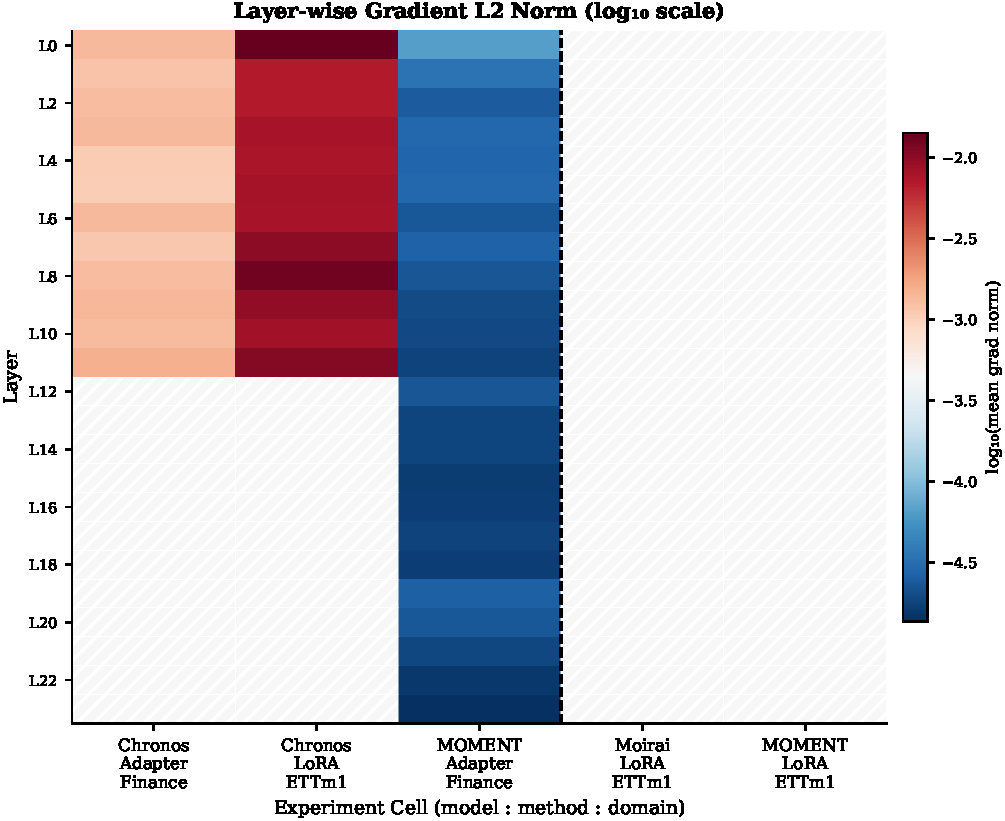
\includegraphics[width=0.85\textwidth]{results/gradient_analysis/figures/gradient_heatmap}
\caption{\textbf{Per-layer gradient magnitude heatmap} across five (model, method, domain) cells (2 seeds, 3 epochs). Chronos+Adapter and Chronos+LoRA on Finance/ETTm1 concentrate gradient energy in early encoder layers; MOMENT+Adapter on Finance distributes flow uniformly across all 24 layers---a qualitative correlate of MOMENT's low method sensitivity. Hatched cells (Moirai+LoRA, MOMENT+LoRA on ETTm1) are NaN due to the LoRA divergence on these cells.}
\label{fig:gradient-heatmap}
\end{figure*}

\begin{figure*}[t]
\centering
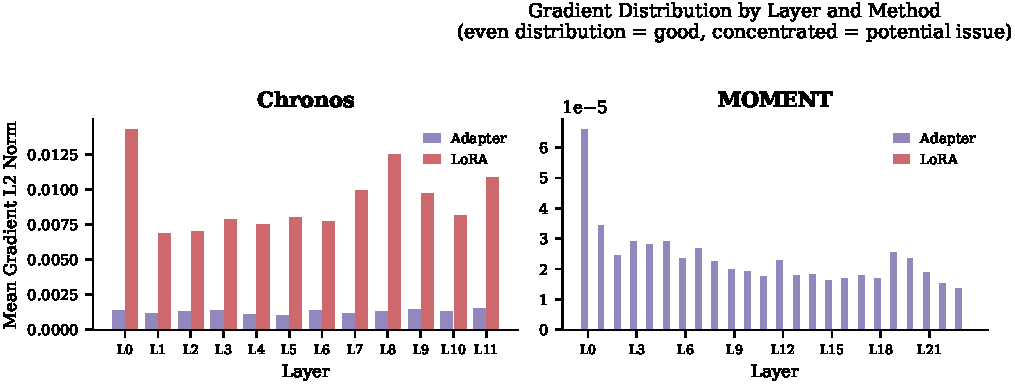
\includegraphics[width=0.85\textwidth]{results/gradient_analysis/figures/gradient_distribution}
\caption{\textbf{Per-layer gradient distributions.} Chronos+Adapter exhibits a multi-modal distribution across the 12 encoder layers; MOMENT+Adapter is unimodal across 24 layers. The distributional difference is qualitatively consistent with the divergent interaction effects ($\eta^2_{\text{int}} = 0.225$ vs.\ $0.000$) observed in the ANOVA; we treat this as a correlate rather than a formal mechanistic test.}
\label{fig:gradient-distribution}
\end{figure*}

%% ================================================================
\section{Spectral--Rank Correlation Analysis (Exploratory)}
\label{sec:spectral-rank}
We explored whether domain shift properties predict optimal rank selection by examining the relationship between spectral Wasserstein distance ($W_1$) of each domain's train$\to$test shift and rank sensitivity (standard deviation of MAE across ranks $\{4,8,16,32\}$). Pearson $\rho = 0.70$ (permutation $p = 0.016$) is significant, but Spearman $\rho_s = 0.27$ ($p = 0.42$) is not. The discrepancy reflects sensitivity to influential points: Chronos+ETTm1 (training divergence, zero rank sensitivity) is a high-leverage observation. Removing it yields Spearman $\rho_s = 0.87$ ($p = 0.012$). We treat this as exploratory evidence that spectral complexity may relate to rank sensitivity, pending validation with more domains.

\begin{figure*}[t]
\centering
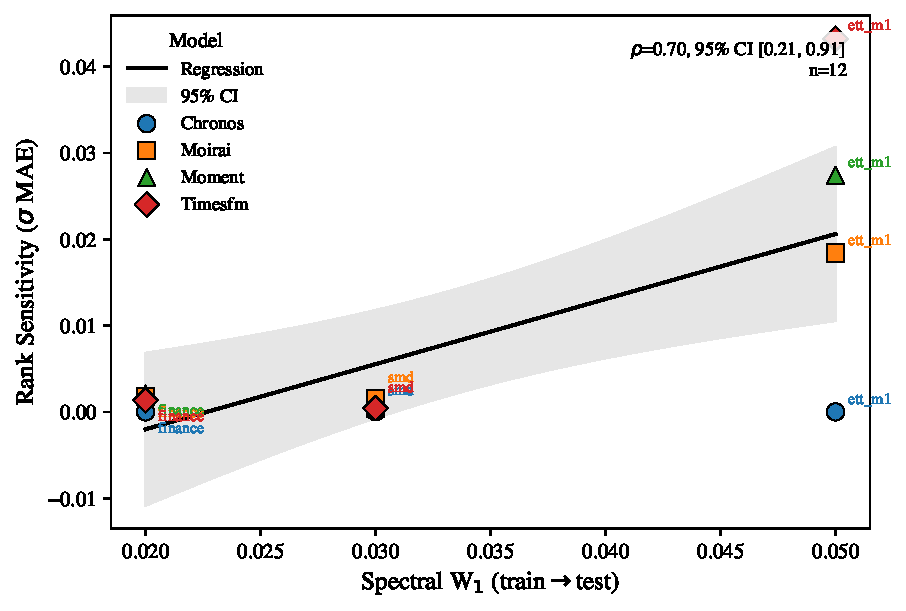
\includegraphics[width=0.7\textwidth]{spectral_rank_scatter.pdf}
\caption{Scatter plot of spectral Wasserstein distance ($W_1$) versus rank sensitivity (std of MAE across ranks $\{4,8,16,32\}$). The linear association is sensitive to influential points, especially Chronos+ETTm1.}
\label{fig:spectral-rank-scatter}
\end{figure*}

%% ================================================================
\section{Selector Design Recipe at Small Grid Sizes}
\label{sec:design-recipe}
Our negative result on granular and learned selectors crystallises a concrete design recipe for the Algorithm Selection Problem at small grids:
\begin{enumerate}[nosep,leftmargin=*]
  \item \textbf{Test the constant-plurality baseline first.} If the oracle distribution is dominated by one method (5/12 cells in our grid), that method is the LODO majority and is hard to beat without exponentially more cells.
  \item \textbf{Diagnose with the marginal vs.\ conditional gap.} If LODO Majority and the best learned selector achieve similar regret (here, $0.015$ vs $0.018$), the binding signal is marginal and granular features will not help.
  \item \textbf{Prefer regularised linear over high-capacity learners} until training-cell count $\gtrsim 5 \cdot n_{\text{methods}}^2$ per LOOCV fold; in our 9-cell folds this threshold ($\approx 125$) is not approached, which explains why decision tree and random forest collapse to $0\%$ top-1.
  \item \textbf{Report regret-based metrics, not top-1 accuracy.} Random matches Arch-Default on top-1 ($33.3\%$ vs $33.3\%$ for non-Pareto-aware oracle) but produces $17\times$ higher regret; rank- and regret-based evaluation surfaces the cost of being wrong.
\end{enumerate}
We expect this recipe to transfer to other small-grid ASP problems---e.g., AutoML for emerging modalities---where the cost of growing the candidate set is comparable to the cost of building a richer training matrix.

%% ================================================================
\section{Hyperparameters and Training Configuration}
\label{sec:hyperparams}
All hyperparameters are stored in \texttt{configs/} as Hydra YAML files; no hyperparameter is hardcoded in the scripts. Table~\ref{tab:hyperparams} summarises the values used for every primary-model run reported in the paper.

\begin{table}[ht]
\centering
\caption{Training and adaptation hyperparameters (identical across architectures unless noted).}
\label{tab:hyperparams}
\small
\begin{tabular}{lll}
\toprule
Group & Hyperparameter & Value \\
\midrule
\multirow{8}{*}{Training}
 & Optimizer       & AdamW \\
 & Learning rate   & $1{\times}10^{-4}$ \\
 & Weight decay    & 0.01 \\
 & Scheduler       & Linear warmup (100 steps) + cosine decay \\
 & Max grad norm   & 1.0 \\
 & Mixed precision & FP16 (Chronos/MOMENT), BF16 (Moirai) \\
 & Batch size      & 32 \\
 & Grad accumulation & 1 \\
 & Max epochs      & 50 \\
 & Early-stopping patience & 10 epochs (val MAE) \\
\midrule
\multirow{4}{*}{LoRA / DoRA}
 & Rank $r$        & 8 (default sweep $\in\{4,8,16,32\}$) \\
 & $\alpha$        & 16 \\
 & Dropout         & 0.05 \\
 & Target modules  & q, k, v, o (\texttt{attn\_all}) \\
\midrule
Adapter (IA$^3$) & Bottleneck size & 64 \\
\midrule
Locus sweep & Insertion points & attn\_qv, attn\_all, ffn, attn\_qv\_ffn, early\_layers, late\_layers \\
\midrule
\multirow{2}{*}{Selection}
 & Best-checkpoint criterion & lowest val MAE \\
 & Final eval split          & domain-specific test partition \\
\bottomrule
\end{tabular}
\end{table}

%% ================================================================
\section{Domain Statistics}
\label{sec:domain-stats}
Table~\ref{tab:domain-stats} reports the structural statistics of each evaluation domain. Note that ETTm1 uses the standard 60/20/20 chronological split, Finance the Autoformer-benchmark 70/10/20 split, SMD a per-machine concatenation with NaN-sentinel boundaries (val carved from the last 20\% of the train concatenation), and PhysioNet a patient-level 70/15/15 split with patient identity preserved across splits.

\begin{table}[ht]
\centering
\caption{Per-domain dataset and forecasting configuration. \emph{Ctx/Hzn}: context length / forecast horizon. \emph{Entity boundary}: whether sliding windows are forbidden from crossing patient/machine boundaries.}
\label{tab:domain-stats}
\footnotesize
\setlength{\tabcolsep}{4pt}
\begin{tabular}{l l l l c l l}
\toprule
Domain & Source & Freq. & Target & Ctx/Hzn & Train/Val/Test & Boundary \\
\midrule
ETTm1     & ETT-small      & 15\,min & OT (oil temp.)  & 512/96 & 60/20/20\%             & N/A \\
Finance   & ExchangeRate   & 1\,day  & col 0 (AUD)     & 96/24  & 70/10/20\%             & N/A \\
SMD       & SMD            & 1\,min  & col 0           & 100/25 & per-machine, val 20\%  & enforced \\
PhysioNet & PhysioNet 2012 & 1\,hr   & HR (heart rate) & 48/12  & 70/15/15\% (patient)   & enforced \\
\bottomrule
\end{tabular}
\end{table}

%% ================================================================
\section{Trainable Parameter Counts}
\label{sec:params}
Table~\ref{tab:params} reports the empirical trainable-parameter percentage per (model, method) cell, averaged over all completed seed-level runs. The pattern explains the architecture-specific efficiency frontier in main-paper Section~4.4: Moirai's IA$^3$ trainable count is two orders of magnitude smaller than Chronos's, and MOMENT's adapter mass is dominated by its head (the model has no dedicated decoder).

\begin{table}[ht]
\centering
\caption{Trainable / total parameter counts and percentage per (model, method). Aggregated over completed runs.}
\label{tab:params}
\small
\begin{tabular}{llrrr}
\toprule
Model & Method & Trainable params & Total params & Trainable \% \\
\midrule
\multirow{6}{*}{Chronos}
 & Zero-shot & 0 & 201,374,976 & 0.0000\% \\
 & Head-only & 0 & 201,374,976 & 0.0000\% \\
 & LoRA      & 1,769,472 & 203,144,448 & 0.8710\% \\
 & DoRA      & 1,880,064 & 203,255,040 & 0.9250\% \\
 & IA$^3$    & 202,752 & 201,577,728 & 0.1006\% \\
 & Full-FT   & 201,374,976 & 201,374,976 & 100.0\% \\
\midrule
\multirow{6}{*}{Moirai}
 & Zero-shot & 0 & 91,357,728 & 0.0000\% \\
 & Head-only & 0 & 91,357,728 & 0.0000\% \\
 & LoRA      & 589,824 & 91,947,552 & 0.6415\% \\
 & DoRA      & 626,688 & 91,984,416 & 0.6813\% \\
 & IA$^3$    & 33,792 & 91,391,520 & 0.0370\% \\
 & Full-FT   & 91,357,728 & 91,357,728 & 100.0\% \\
\midrule
\multirow{6}{*}{MOMENT}
 & Zero-shot & 0 & 341,231,104 & 0.0000\% \\
 & Head-only & 6,291,552 & 341,231,104 & 1.8438\% \\
 & LoRA      & 7,864,416 & 342,803,968 & 2.2941\% \\
 & DoRA      & 7,962,720 & 342,902,272 & 2.3222\% \\
 & IA$^3$    & 6,457,440 & 341,396,992 & 1.8915\% \\
 & Full-FT   & 347,522,656 & 341,231,104 & 100.0\%$^\dagger$ \\
\bottomrule
\multicolumn{5}{l}{\scriptsize $^\dagger$MOMENT Full-FT trainable count includes the forecasting head not present in zero-shot total.} \\
\end{tabular}
\end{table}

%% ================================================================
\section{Per-cell mean MAE (full grid)}
\label{sec:per-cell-mae}
Table~\ref{tab:per-cell-mae} reports the per-cell mean MAE (averaged over completed seeds, after the per-cell scale-aware outlier filter) for every (model, method, domain) combination in the primary inference set. Each cell is the value entering the per-architecture ANOVA reported in main-paper Table~3.

\begin{table}[ht]
\centering
\caption{Per-cell mean MAE for primary models, after per-cell outlier filtering. ``---'' marks fully diverged cells (all seeds excluded).}
\label{tab:per-cell-mae}
\small
\begin{tabular}{lllrrrr}
\toprule
Model & Method & ETTm1 & Finance & SMD & PhysioNet \\
\midrule
\multirow{6}{*}{Chronos}
 & Zero-shot & 1.1449 & 0.0208 & 0.0238 & 15.16 \\
 & Head-only & 0.2178 & 0.0038 & 0.0084 & 5.33 \\
 & LoRA      & ---    & 0.0038 & 0.0099 & 18.82 \\
 & DoRA      & 2.3178 & 0.0038 & 0.0040 & 15.65 \\
 & IA$^3$    & 0.2152 & 0.0038 & 0.0084 & 5.24 \\
 & Full-FT   & 0.2275 & 0.0038 & 0.0083 & --- \\
\midrule
\multirow{6}{*}{Moirai}
 & Zero-shot & 3.8475 & 0.0871 & 0.0927 & 44.28 \\
 & Head-only & 1.4313 & 0.0250 & 0.0322 & 15.76 \\
 & LoRA      & 1.3804 & 0.0273 & 0.0354 & --- \\
 & DoRA      & 1.3789 & 0.0270 & 0.0206 & 16.93 \\
 & IA$^3$    & 1.2599 & 0.0250 & 0.0182 & 15.64 \\
 & Full-FT   & 1.2326 & 0.0223 & 0.0357 & 16.20 \\
\midrule
\multirow{6}{*}{MOMENT}
 & Zero-shot & 2.2262 & 0.0687 & 0.0645 & 15.59 \\
 & Head-only & 1.3763 & 0.0279 & 0.0294 & 15.14 \\
 & LoRA      & 1.3675 & 0.0280 & 0.0295 & 15.11 \\
 & DoRA      & 1.6134 & 0.0289 & 0.0168 & 15.07 \\
 & IA$^3$    & 1.3799 & 0.0273 & 0.0298 & 15.17 \\
 & Full-FT   & 1.3827 & 0.0282 & 0.0299 & 15.14 \\
\bottomrule
\end{tabular}
\end{table}

%% ================================================================
\section{Selector per-fold breakdown}
\label{sec:selector-fold}
Main-paper Table~6 reports selector summary statistics aggregated over 4 LOOCV folds. Table~\ref{tab:selector-fold} reports per-fold top-1 hits and mean regret for the five most-discussed strategies. The fold breakdown shows that LODO Majority's strength is concentrated in the PhysioNet fold (2/3 cells correct) and that Logistic Meta matches LODO on 3 of 4 folds; the divergent fold is SMD, where Arch-Default and Regret-W NN suffer their largest regret (0.33). The single-fold variability illustrates why we treat the $n{=}12$ headline as directional.

\begin{table}[ht]
\centering
\caption{Per-fold selector breakdown: top-1 hits (out of 3 cells) and mean regret per held-out domain.}
\label{tab:selector-fold}
\small
\begin{tabular}{ll cccc}
\toprule
Strategy & Metric & ETTm1 & Finance & PhysioNet & SMD \\
\midrule
\multirow{2}{*}{LODO Majority}
 & top-1 hits & 1/3 & 1/3 & 2/3 & 1/3 \\
 & mean regret & 0.010 & 0.041 & 0.001 & 0.009 \\
\midrule
\multirow{2}{*}{Arch-Default}
 & top-1 hits & 0/3 & 0/3 & 2/3 & 0/3 \\
 & mean regret & 0.014 & 0.050 & 0.012 & 0.327 \\
\midrule
\multirow{2}{*}{Regret-W NN}
 & top-1 hits & 1/3 & 1/3 & 2/3 & 1/3 \\
 & mean regret & 0.010 & 0.041 & 0.001 & 0.327 \\
\midrule
\multirow{2}{*}{Logistic Meta}
 & top-1 hits & 1/3 & 1/3 & 1/3 & 1/3 \\
 & mean regret & 0.010 & 0.041 & 0.013 & 0.009 \\
\midrule
\multirow{2}{*}{Decision-Tree}
 & top-1 hits & 0/3 & 0/3 & 0/3 & 0/3 \\
 & mean regret & 0.029 & 0.048 & 0.878 & 0.327 \\
\bottomrule
\end{tabular}
\end{table}

%% ================================================================
\section{Datasheet for TSFM-PEFT-Bench}
\label{sec:datasheet}
We include a datasheet~\citep{gebru2021datasheets} for TSFM-PEFT-Bench. The full machine-readable description is in the Croissant 1.0 manifest \texttt{tsfm\_peft\_bench.croissant.json} (RAI fields populated). This section provides the human-readable answers to the standard questions.

\paragraph{Motivation.} TSFM-PEFT-Bench was created to answer whether parameter-efficient fine-tuning (PEFT) recommendations are reliable across time series foundation model (TSFM) architectures and domains. Prior PEFT studies for TSFMs each fixed either the model or the domain, making it impossible to disentangle method, architecture, and domain effects. The benchmark was created by the authors as part of the paper that this Appendix accompanies.

\paragraph{Composition.} Each instance is a single training-and-evaluation run identified by (model, method, domain, seed[, rank, locus]). We release 882 paper-included primary-model runs (3 TSFMs $\times$ 4 domains $\times$ 6 main methods + rank/locus sweeps) plus 90 TimesFM descriptive runs (972 total). Each record contains: experiment\_id, model, method, domain, seed, rank, locus, metrics (MAE, MSE, MASE where available), trainable\_params, total\_params, train\_loss\_final, val\_loss\_best, epochs\_trained, gpu\_memory\_mb, train\_time\_seconds, and the Hydra-resolved config. There are no labels or human annotations; each record is the deterministic output of \texttt{scripts/run\_expansion.py}.

\paragraph{Collection process.} Runs were generated on a heterogeneous compute pool (4$\times$ NVIDIA RTX 3090 + 40$\times$ RTX 3060 cluster nodes) over approximately 2{,}250 GPU-hours between 2026-01 and 2026-04. Pre-trained TSFM checkpoints were loaded from the public Hugging Face Hub. Source domain CSVs are publicly available (ETT-small, exchange\_rate, SMD, PhysioNet 2012). No human-subject data is collected; PhysioNet 2012 inputs are de-identified ICU heart-rate sequences and we use only the HR target column at hourly resolution.

\paragraph{Preprocessing / cleaning / labeling.} Per-domain context/horizon and split ratios are stored in \texttt{configs/data/*.yaml} and summarised in Appendix~\ref{sec:domain-stats}. SMD uses a 50{,}000-row contiguous prefix after machine concatenation with NaN-sentinel boundaries; PhysioNet's long-context DoRA branch uses \texttt{enforce\_entity\_boundary=False} (relaxed window concatenation across patient boundaries while preserving labels). The analysis pipeline applies a per-cell scale-aware outlier filter (MAE${>}10\times$ same-(model, domain) zero-shot baseline) for the inferential analyses; raw runs are released without filtering so users can apply alternative rules.

\paragraph{Uses.} Intended uses: (i) reproducing and auditing PEFT-recommendation claims across TSFM architectures; (ii) developing and evaluating selector strategies for PEFT method recommendation under domain shift; (iii) studying methodological pitfalls in cross-domain evaluation; (iv) downstream meta-learning research at small evaluation grids; (v) educational use as an example of cross-architecture empirical audit. The dataset must \emph{not} be used to claim that any single PEFT method is universally best, since the benchmark is explicitly designed to refute such claims.

\paragraph{Distribution.} The benchmark is hosted as described in the README's Hosting section. Code is mirrored on Anonymous-4-Open-Science during review; the run manifest, headline numbers, and per-run JSONs are bundled in the supplementary tarball. After acceptance, both code and run JSONs will be released on Hugging Face under Apache-2.0. The Croissant manifest enables programmatic loading.

\paragraph{Maintenance.} The authors commit to maintaining the benchmark at least until NeurIPS 2027, including bug fixes, rerun requests, and documentation improvements. Versioning is via git tags. Issues are reported via the repository tracker.

\paragraph{Personal and sensitive information.} PhysioNet 2012 contains de-identified ICU heart-rate time series; we use only the aggregate HR forecasting metric and do not redistribute raw patient records. ETTm1, exchange\_rate, and SMD contain no human-subject data. The benchmark records (per-run JSONs) expose only forecasting metrics and config metadata, no PII.

\paragraph{Biases and limitations.} See Section~\ref{sec:limitations} of the main paper and \texttt{rai:dataLimitation} / \texttt{rai:dataBiases} in the Croissant file. Key items: 12-cell evaluation grid; plurality dependence on IA$^3$; uneven Moirai coverage; per-domain absolute MAE not directly comparable; selection bias in architectures (3 publicly available TSFMs that admit all considered PEFT methods) and methods (5 main + DoRA + descriptive Prefix; FourierFT and BitFit not evaluated); MASE coverage 35\%.

\paragraph{License.} Code: Apache-2.0 (\texttt{LICENSE}). Run manifest and per-run JSONs: Apache-2.0. Source dataset licenses are documented in the Reproducibility Statement (Section~\ref{sec:repro}); we do not redistribute raw source data.

%% ================================================================
\section{Reproducibility Statement}
\label{sec:repro}

\paragraph{Code.} All experiment scripts, model wrappers, and analysis pipelines will be released upon acceptance. The codebase provides two entry points: (1)~\texttt{scripts/train.py}, a Hydra-based entry point for single-run experiments (e.g., \texttt{python scripts/train.py model=chronos adaptation=lora data=ett\_m1}); and (2)~\texttt{scripts/run\_expansion.py}, the orchestrator used to execute the full experiment matrix reported in the paper (e.g., \texttt{python scripts/run\_expansion.py --models chronos,moment,moirai --mode domain --seeds 42,123,7,2024,3407}). All results in the paper were produced via \texttt{run\_expansion.py}; \texttt{train.py} serves as a development/debugging entry point for individual configurations (Chronos and MOMENT only; not all method--model combinations are supported). Analysis scripts (\texttt{analyze\_expansion\_v2.py}, \texttt{generate\_neurips\_figures.py}) consume the JSON outputs produced by \texttt{run\_expansion.py}.

\paragraph{Data.} ETTm1~\citep{zhou2021ett}, Finance (\texttt{exchange\_rate})~\citep{li2019logsparse}, SMD~\citep{su2019robust}, and PhysioNet 2012~\citep{silva2012physionet} are publicly available.

\paragraph{Computing.} Experiments were conducted on a mixed pool: 4$\times$ NVIDIA RTX 3090 (24\,GB each) for the primary experiment matrix, with an additional 40 RTX 3060 (12\,GB) nodes from a shared cluster used for DoRA supplementary runs and gradient probe experiments. All models use FP16/BF16 precision. Total wall-clock compute at submission time: approximately 2,250 GPU-hours across 972 completed runs (882 paper-included primary-model runs plus 90 TimesFM descriptive runs). Per-run times range from ${\sim}$6 minutes (MOMENT zero-shot) to ${\sim}$6.5 hours (Chronos LoRA on RTX 3090); RTX 3060 runs are $3$--$5\times$ slower at the same batch size.

\paragraph{Random seeds.} The planned seed set is $\{42, 123, 7, 2024, 3407\}$. Completed runs are a subset of this target for several Chronos and Moirai configurations, as summarized in Table~\ref{tab:seed-coverage}.

\paragraph{Software.} Python 3.12, PyTorch 2.4.1, HuggingFace Transformers, PEFT (LoRA/IA$^3$), and statsmodels for ANOVA. Chronos~\citep{ansari2024chronos}, MOMENT~\citep{goswami2024moment}, and Moirai~\citep{woo2024moirai} are loaded from Hugging Face Hub. TimesFM~\citep{das2024timesfm} is unavailable in our environment due to a \texttt{paxml}/\texttt{lingvo} dependency conflict.

\paragraph{Assets and licenses.} We explicitly track the upstream assets used in the study. The model checkpoints \texttt{amazon/chronos-t5-base} and \texttt{google/timesfm-1.0-200m} are distributed under Apache-2.0, \texttt{AutonLab/MOMENT-1-large} under MIT, and \texttt{Salesforce/moirai-1.1-R-base} under CC-BY-NC-4.0 according to their Hugging Face model cards. For datasets, the ETT repository reports CC-BY-ND-4.0 for ETTm1. In contrast, the \texttt{laiguokun/multivariate-time-series-data} repository used for the Exchange Rate benchmark does not expose a repository-level license file or dataset-specific license text that we could verify at submission time, and the prepared benchmark package does not clearly inherit a standalone license from the underlying public exchange-rate sources. Likewise, the OmniAnomaly repository is MIT-licensed for code, but we could not verify any authoritative statement that this code license also governs the bundled Server Machine Dataset collected from an Internet company. We therefore cite and credit all upstream assets, but conservatively mark checklist compliance for asset-license completeness as partial rather than complete.

\paragraph{LLM-assisted writing and code review (transparency note).} Anthropic's Claude and OpenAI's Codex assisted with (i)~English drafting and LaTeX source editing/auditing, (ii)~academic-style polishing, and (iii)~Python code review and error fixes for author-identified bug patches. These tools did not design experiments, generate empirical results, choose baselines, or alter any reported number; all scientific decisions and final wording are the authors' responsibility. Per the NeurIPS 2026 LLM policy, this usage falls under writing-assistance/basic-code-assistance categories that do not require disclosure; we include it here for transparency.

%% ================================================================
\section{Broader Impacts}
\label{sec:broader}
This work studies how to adapt forecasting and anomaly-oriented time series foundation models more reliably under domain shift. Positive impacts include reducing wasted compute from brittle adaptation choices and improving robustness in high-stakes domains such as healthcare, energy, and industrial monitoring. Negative impacts include overconfidence in model transfer across domains and potential misuse in surveillance-heavy settings if anomaly detection models are deployed without appropriate human oversight. We therefore recommend domain-specific validation before deployment and transparent reporting of adaptation failures.


\clearpage
\section*{NeurIPS Paper Checklist}

\begin{enumerate}

\item {\bf Claims}
    \item[] Question: Do the main claims made in the abstract and introduction accurately reflect the paper's contributions and scope?
    \item[] Answer: \answerYes{}
    \item[] Justification: The abstract and introduction state the main claims as a cross-architecture empirical audit: significant Method$\times$Domain interaction, unstable cross-domain method transfer, and architecture-specific efficiency tradeoffs. Representation-similarity analysis is explicitly framed as preliminary diagnostic evidence rather than as a primary claim.

\item {\bf Limitations}
    \item[] Question: Does the paper discuss the limitations of the work performed by the authors?
    \item[] Answer: \answerYes{}
    \item[] Justification: Limitations are discussed in Section~5 under a dedicated paragraph. These include limited domain coverage, uneven seed coverage across methods, the preliminary status of CKA diagnostics, the treatment of divergence outliers, partial MASE coverage, and the small $n{=}12$ LODO evaluation grid.

\item {\bf Theory assumptions and proofs}
    \item[] Question: For each theoretical result, does the paper provide the full set of assumptions and a complete (and correct) proof?
    \item[] Answer: \answerNA{}
    \item[] Justification: The paper does not present formal theoretical results, theorems, or proofs; it is an empirical benchmarking and analysis study.

\item {\bf Experimental result reproducibility}
    \item[] Question: Does the paper fully disclose all the information needed to reproduce the main experimental results of the paper to the extent that it affects the main claims and/or conclusions of the paper (regardless of whether the code and data are provided or not)?
    \item[] Answer: \answerYes{}
    \item[] Justification: Section~3 and the appendix reproducibility statement specify datasets, model families, adaptation methods, ranks, loci, statistical tests, compute setup, planned seeds, completed-run accounting, software versions, and Hydra-based training entry points needed to reproduce the reported analyses.

\item {\bf Open access to data and code}
    \item[] Question: Does the paper provide open access to the data and code, with sufficient instructions to faithfully reproduce the main experimental results, as described in supplemental material?
    \item[] Answer: \answerYes{}
    \item[] Justification: Code, configs, run manifest, headline-number artifacts, and the Croissant 1.0 manifest are released for review via an anonymous URL (\texttt{https://anonymous.4open.science/r/tsfm-peft-bench-anon}), and the supplementary tarball bundles the same artifacts plus per-run JSONs. The Reproducibility Statement (Appendix~\ref{sec:repro}) and Datasheet (Appendix~\ref{sec:datasheet}) describe the exact reproduction commands. Source datasets are publicly available; the README documents per-platform hosting plans for camera-ready release.

\item {\bf Experimental setting/details}
    \item[] Question: Does the paper specify all the training and test details (e.g., data splits, hyperparameters, how they were chosen, type of optimizer) necessary to understand the results?
    \item[] Answer: \answerYes{}
    \item[] Justification: Section~3 describes datasets, adaptation axes, experiment scale, and the primary statistical methodology. The appendix reproducibility statement adds hardware, software versions, the planned seed set, completed observation counts, and the Hydra entry points used to launch training.

\item {\bf Experiment statistical significance}
    \item[] Question: Does the paper report error bars suitably and correctly defined or other appropriate information about the statistical significance of the experiments?
    \item[] Answer: \answerYes{}
    \item[] Justification: The main claims are supported by ANOVA $F$-statistics and $\eta^2$ effect sizes, mean$\pm$std MAE in the efficiency table, and Wilson confidence intervals for the LODO transfer experiment. The appendix additionally reports ANOVA degrees of freedom and exploratory robustness analyses.

\item {\bf Experiments compute resources}
    \item[] Question: For each experiment, does the paper provide sufficient information on the computer resources (type of compute workers, memory, time of execution) needed to reproduce the experiments?
    \item[] Answer: \answerYes{}
    \item[] Justification: The appendix reproducibility statement reports the hardware (4$\times$ RTX 3090, 24\,GB each), precision (FP16/BF16), approximate total compute (${\sim}$2,250 GPU-hours across 885 completed runs), and software stack. Table~\ref{tab:efficiency} reports per-run wall-clock time by method.

\item {\bf Code of ethics}
    \item[] Question: Does the research conducted in the paper conform, in every respect, with the NeurIPS Code of Ethics \url{https://neurips.cc/public/EthicsGuidelines}?
    \item[] Answer: \answerYes{}
    \item[] Justification: The work is an empirical analysis of public datasets and pre-trained models, with no human subjects or sensitive data collection. The submission preserves anonymity and discusses failure modes and deployment caution in the appendix broader impacts section.

\item {\bf Broader impacts}
    \item[] Question: Does the paper discuss both potential positive societal impacts and negative societal impacts of the work performed?
    \item[] Answer: \answerYes{}
    \item[] Justification: The appendix broader impacts section discusses positive impacts (more reliable adaptation, reduced wasted compute) and negative impacts (overconfident transfer under domain shift, potential surveillance misuse), together with the mitigation recommendation of domain-specific validation before deployment.

\item {\bf Safeguards}
    \item[] Question: Does the paper describe safeguards that have been put in place for responsible release of data or models that have a high risk for misuse (e.g., pre-trained language models, image generators, or scraped datasets)?
    \item[] Answer: \answerNA{}
    \item[] Justification: The paper does not release a new model, scraped dataset, or dual-use asset. It analyzes adaptation behavior of existing public models and datasets.

\item {\bf Licenses for existing assets}
    \item[] Question: Are the creators or original owners of assets (e.g., code, data, models), used in the paper, properly credited and are the license and terms of use explicitly mentioned and properly respected?
    \item[] Answer: \answerYes{}
    \item[] Justification: The appendix enumerates verified upstream licenses (Apache-2.0 for Chronos/TimesFM, MIT for MOMENT, CC-BY-NC-4.0 for Moirai, CC-BY-ND-4.0 for ETTm1). The Exchange Rate benchmark and the bundled SMD code are clearly credited to their upstream maintainers (\texttt{laiguokun/multivariate-time-series-data} and \texttt{NetManAIOps/OmniAnomaly}); we use them under the upstream repositories' code licenses (MIT) and do not redistribute raw source data. Our own contributions (code, manifest, Croissant file) are released under Apache-2.0. Asset-license caveats for the two upstream sources without standalone dataset license files are documented transparently in the Reproducibility Statement.

\item {\bf New assets}
    \item[] Question: Are new assets introduced in the paper well documented and is the documentation provided alongside the assets?
    \item[] Answer: \answerYes{}
    \item[] Justification: We introduce \textbf{TSFM-PEFT-Bench}, a benchmark of 882 paper-included primary-model PEFT runs (972 total). Documentation includes: a Croissant 1.0 manifest with mandatory Responsible-AI metadata (\texttt{tsfm\_peft\_bench.croissant.json}); a datasheet following~\citet{gebru2021datasheets} (Appendix~\ref{sec:datasheet}); per-domain statistics (Appendix~\ref{sec:domain-stats}); hyperparameters (Appendix~\ref{sec:hyperparams}); per-cell raw MAE (Appendix~\ref{sec:per-cell-mae}); trainable parameter counts (Appendix~\ref{sec:params}); reproducibility statement (Appendix~\ref{sec:repro}); and an \texttt{LICENSE} file (Apache-2.0). Hosting plan is documented in the README.

\item {\bf Crowdsourcing and research with human subjects}
    \item[] Question: For crowdsourcing experiments and research with human subjects, does the paper include the full text of instructions given to participants and screenshots, if applicable, as well as details about compensation (if any)?
    \item[] Answer: \answerNA{}
    \item[] Justification: The research does not involve crowdsourcing or experiments with human subjects.

\item {\bf Institutional review board (IRB) approvals or equivalent for research with human subjects}
    \item[] Question: Does the paper describe potential risks incurred by study participants, whether such risks were disclosed to the subjects, and whether Institutional Review Board (IRB) approvals (or an equivalent approval/review based on the requirements of your country or institution) were obtained?
    \item[] Answer: \answerNA{}
    \item[] Justification: The research does not involve human subjects, so IRB approval is not applicable.

\item {\bf Declaration of LLM usage}
    \item[] Question: Does the paper describe the usage of LLMs if it is an important, original, or non-standard component of the core methods in this research? Note that if the LLM is used only for writing, editing, or formatting purposes and does \emph{not} impact the core methodology, scientific rigor, or originality of the research, declaration is not required.
    \item[] Answer: \answerNA{}
    \item[] Justification: LLMs were not used as part of the core methodology, experiments, or scientific claims. For transparency, the Reproducibility Statement (Appendix~\ref{sec:repro}) records that Anthropic's Claude and OpenAI's Codex assisted only with English drafting/LaTeX editing, academic-style polishing, and Python code review/bug-patch assistance; these tools did not design experiments, generate empirical results, choose baselines, or alter any reported number. Per the NeurIPS 2026 LLM policy, this usage is exempt from disclosure; we declare it nonetheless.

\end{enumerate}


\end{document}
